% !TEX root = ../thesis.tex
\chapter{Project Research}
\label{chap:research}
We've previously seen that ``Tone \& Sculpt'' is an existing similar application
on the market. Below we'll consider other background research on existing
systems and their functionality.

The bulk of fitness mobile applications fall into 2 categories:
\begin{enumerate}
	\item Applications which allow fitness enthusiasts to monitor their training
	      and nutrition - the market leaders in this space
	      (by monthly active users) are ``Fitbit''
	      and ``My Fitness Pal'' (as of March 2018) \cite{statista-monthly-users}.
	\item Applications which allow trainers to facilitate the delivery of programmes
	      either by partnering with the development company or white-labelling software.
	      These are apps focused on trainers more than end users - the most notable player
	      in this emerging market would be ``TrueCoach''\href{https://truecoach.co/} , who
	      raised USD 2.6 million in seed round funding before being
	      acquired by TSG (Transaction Services Group) in April 2020 \cite{truecoach-funding}.
	      Estimated revenue over USD 1.2 million (from 20k users) for 2021 \cite{truecoach-revenue}.
\end{enumerate}

We can see the main difference in these groups are that
the focus of the former is B2C (business-to-consumer) services
whereas the latter focus on B2B (business-to-business; often acting as SaaS companies).
This is an important distinction as \textit{the project} is looking to combine elements
of both and so the following research will reflect this.
\par
We'll also look at vertical jump calculators and the mathematics involved in developing
something of that nature.
\pagebreak

\section{Existing fitness application systems}
We'll look at 4 systems, 2 from each of the aforementioned application groups. Here it is
worth mentioning that some apps are on the borderline such as
``Centr by Chris Hemsworth''\href{https://centr.com/}. The app follows a B2C approach
but is marketed and part-owned by Chris Hemsworth, with his trainers being the facilitators of programmes
and nutrition plans. A similar approach to the aforementioned
\hyperref[sec:intro_motivation]{``female-focused Tone \& Sculpt''}.
Because cases like these are not relevant to the application being built
for the project, we will not look in any depth at these.
\par
For each of these systems we'll be looking at:
\begin{itemize}
	\item A typical user story for the given application.
	\item A high-level breakdown of the system(s) functionality.
	\item A look at the technology in use (where possible).
\end{itemize}
We'll then compare the applications (in pairs) to see any unique features
and to understand which functions are seemingly core to a positive user experience
in the fitness application space.

\subsection{MyFitnessPal}
\begin{figure}[H]
    \centering
    \begin{minipage}{0.5\textwidth}
        \centering
        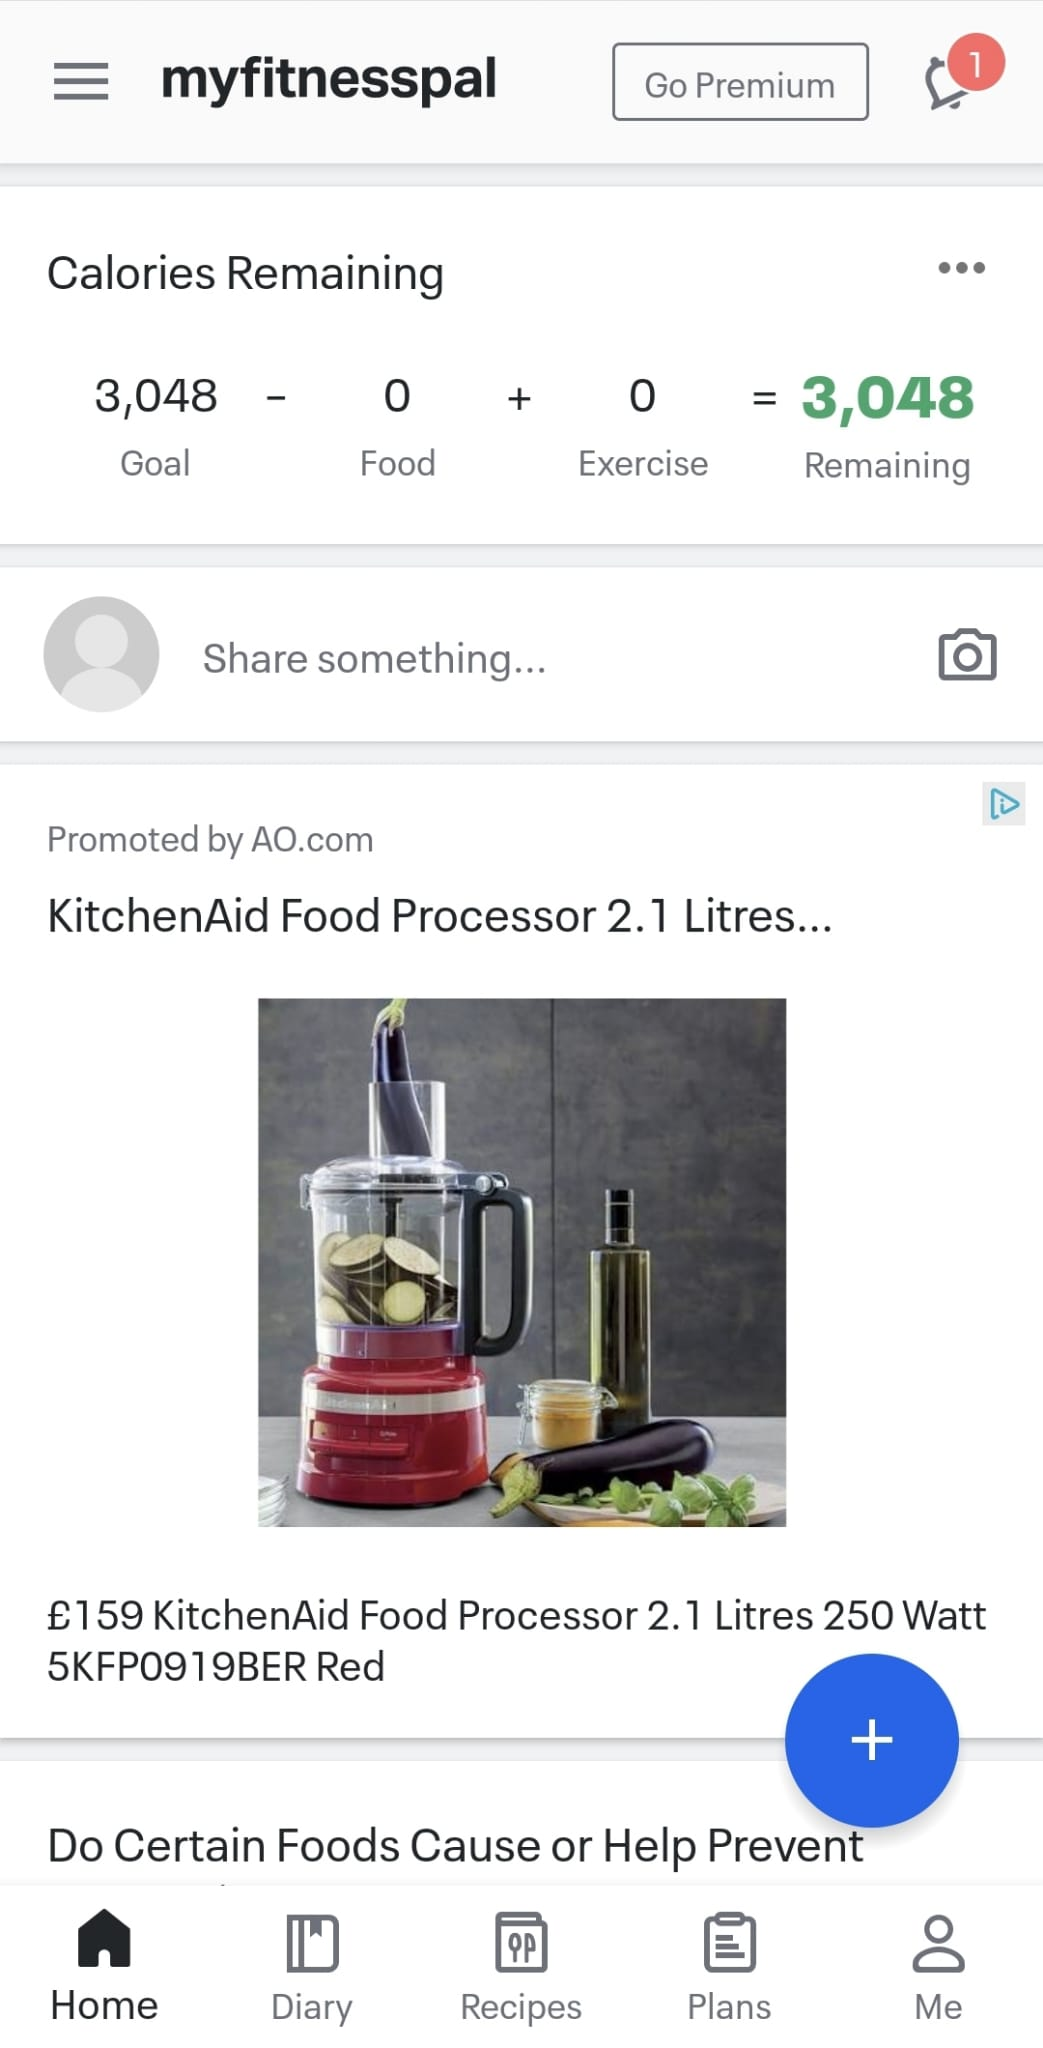
\includegraphics[width=0.5\textwidth]{myfitnesspal/homepage.jpeg}
        \caption{Homepage feed}
        \label{fig:mfp-home}
    \end{minipage}%
    \begin{minipage}{0.5\textwidth}
        \centering
        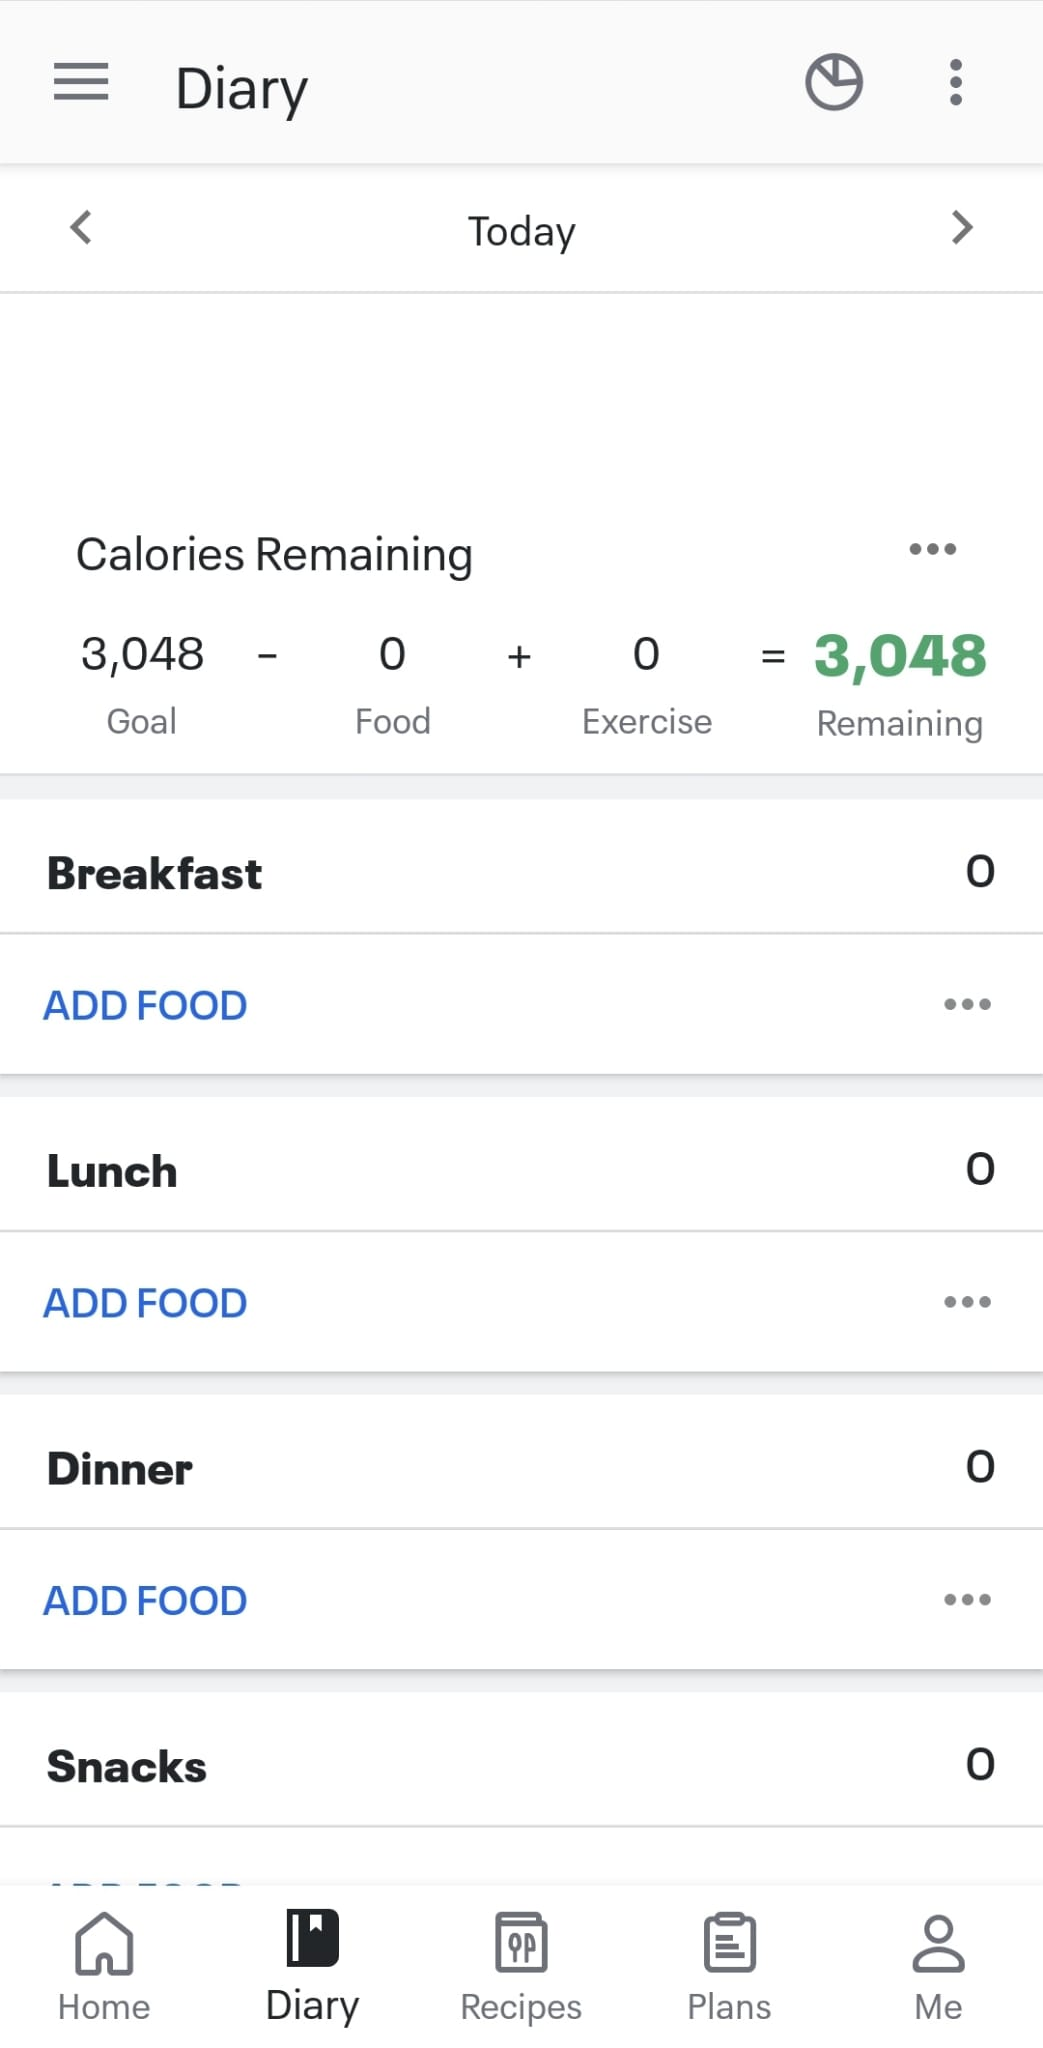
\includegraphics[width=0.5\textwidth]{myfitnesspal/calorie-counter.jpeg}
        \caption{Food diary \& calorie counter}
        \label{fig:mfp-diary}
    \end{minipage}%
\end{figure}
\textbf{User Story}
\label{research-breakdown:mfp-usr-story}
\par
``As a fitness enthusiast, I sign up to the app via email. I wake up
every day and log my breakfast by scanning barcodes for my food.
This is accounted for in my daily food tracking (\cref{fig:mfp-diary}).
After breakfast I create a new workout based on advice from my community or homepage,
I search for the exercises involved and log my workout later on in the day (\cref{fig:mfp-screens}).''
\begin{figure}[H]
    \begin{minipage}{0.5\textwidth}
        \centering
        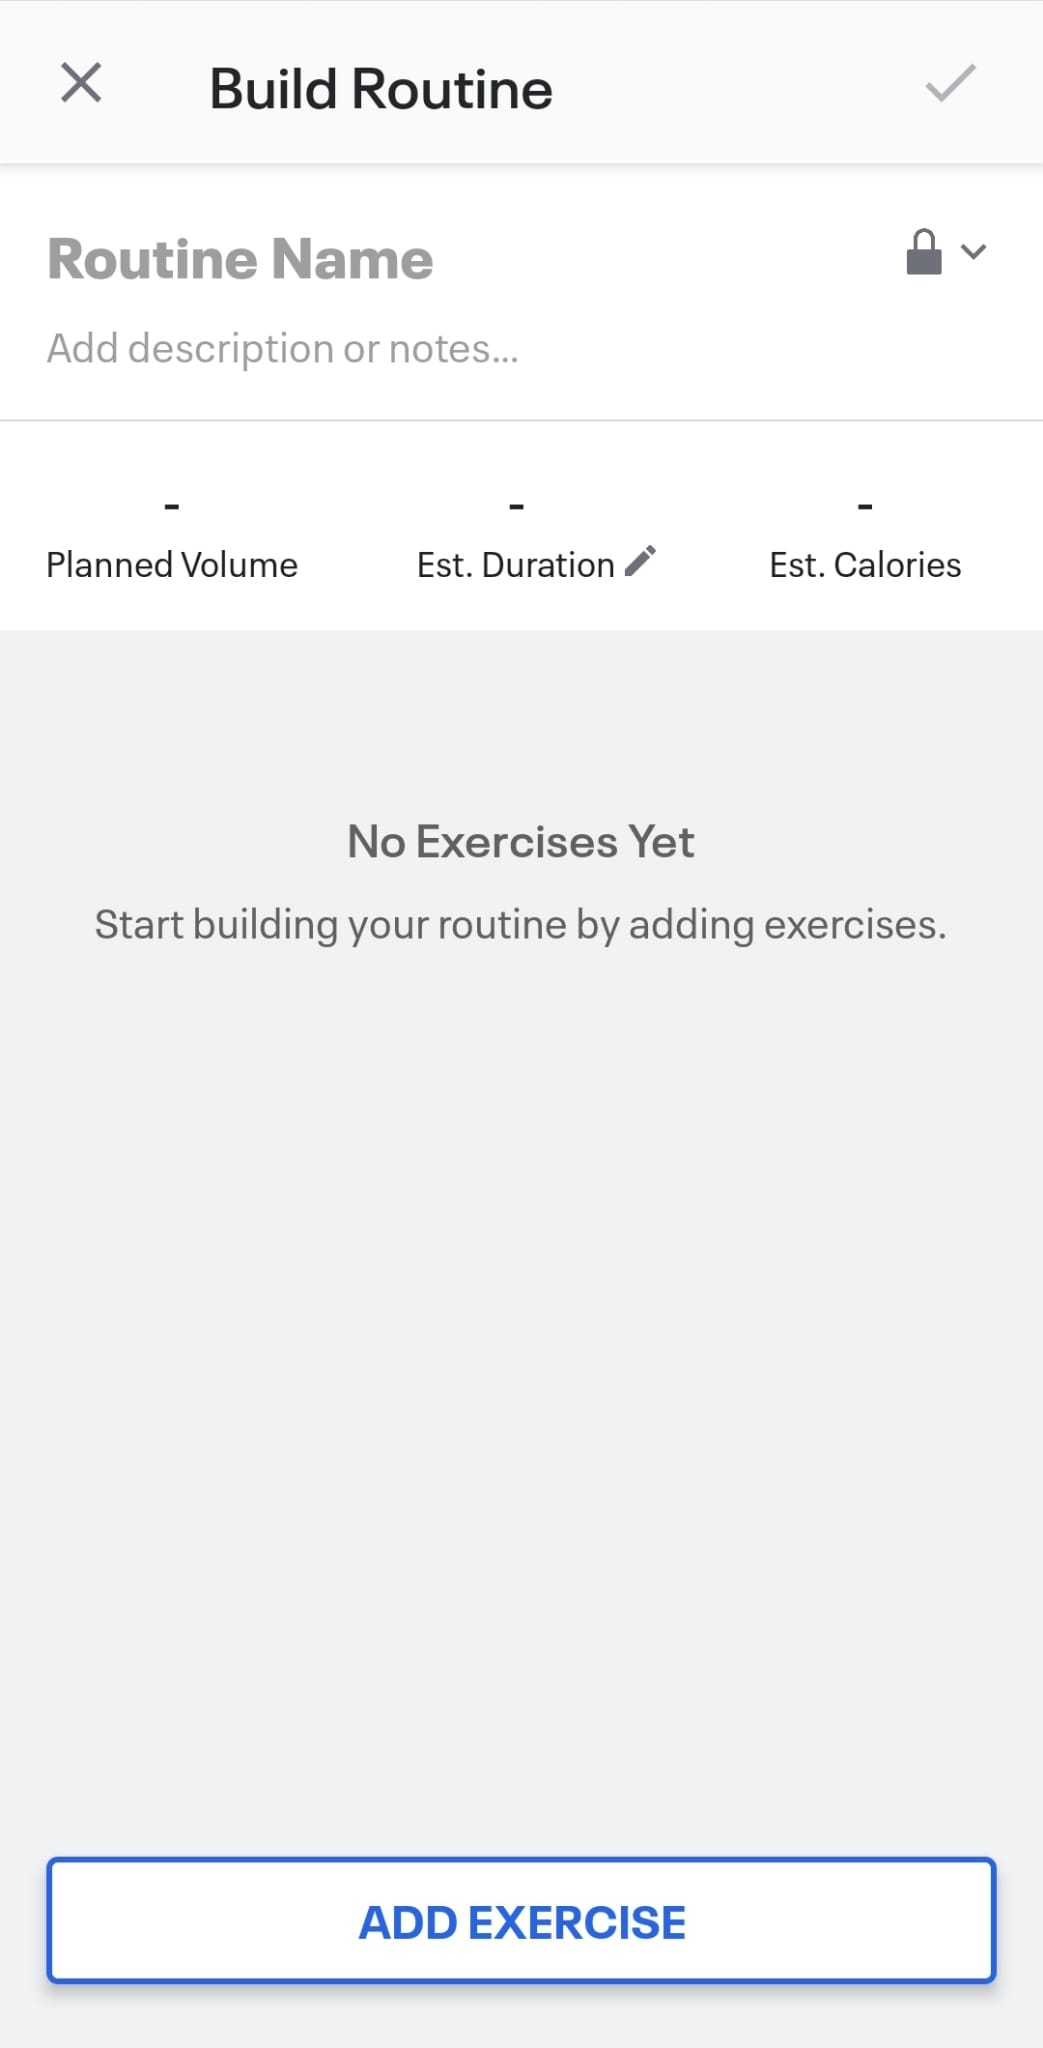
\includegraphics[width=0.5\textwidth]{myfitnesspal/exercise-routines.jpeg}
        \label{fig:mfp-workouts}
    \end{minipage}%
    \begin{minipage}{0.5\textwidth}
        \centering
        \includegraphics[width=0.5\textwidth]{myfitnesspal/exercise-choice.jpeg}
        \label{fig:mfp-exercise-picker}
    \end{minipage}
    \captionof{figure}{The custom workout routines in MFP}
    \label{fig:mfp-screens}
\end{figure}
\textbf{Features/Functionality}
\label{research-breakdown:mfp-features}
\par
MyFitnessPal includes all of the following features:
\begin{multicols}{2}
	\setlist{nolistsep}
	\begin{itemize}[noitemsep]
		\item Estimate calories burned given a set of exercises/a routine.
		\item Track food intake via barcode scan or recipe input.
		\item Track water.
		\item Workout plans provided by MFP.
		\item Track weight.
		      \columnbreak
		\item Create custom workout plans from existing exercises.
		      \setlist{nolistsep}
		      \begin{itemize}[noitemsep]
			      \item Exercises don't include video/images and no ability to add custom exercises.
			      \item These can be shared publically to dashboard.
		      \end{itemize}
		\item Count steps (using compatible devices).
		\item Add friends and send/receive messages.
		\item Community tab (requires separate signup).
		\item Export progress as CSV.
		\item Meal and weight tracking reminders (via push notifications).
		\item Set workout/week, minutes/workout and ``calories burned'' goals.
		\item Discover recipes/meal plans via community and MFP suggestions.
	\end{itemize}
\end{multicols}
\textbf{Technology Stack}
\label{research-breakdown:mfp-stack}
\par
MyFitnessPal uses the following technologies according to Stackshare \cite{mfp-stack}:
\begin{itemize}
	\item React (a JavaScript framework for creating cross-platform applications)
	\item Cloudflare (for web infrastructure)
	\item NginX (for server side use)
	\item Vanilla JavaScript and CSS + libraries (jQuery, Bootstrap)
\end{itemize}
Various other technologies are being used on the server-side but for \textit{the project}
we are primarily concerned with the technology used for the application
as opposed to the backend infrastructure.


\subsection{Fitbit}
Fitbit is the app that accompanies many of the Fitbit brands'
hardware products, their first movers advantage was likely
a large contributor towards their large market share (in 2018)\footnote{Q3 2020 wearables market share = 2.6\%\cite{fitbit-market-share}}
in the application space.
The functionality of their hardware products (which had been the standard for
fitness tracking wearables)
is enhanced through use of the app. The research will consider the application alone and disregard
any wearable-specific functionality.
\pagebreak
\begin{figure}[H]
    \begin{minipage}{0.5\textwidth}
        \centering
        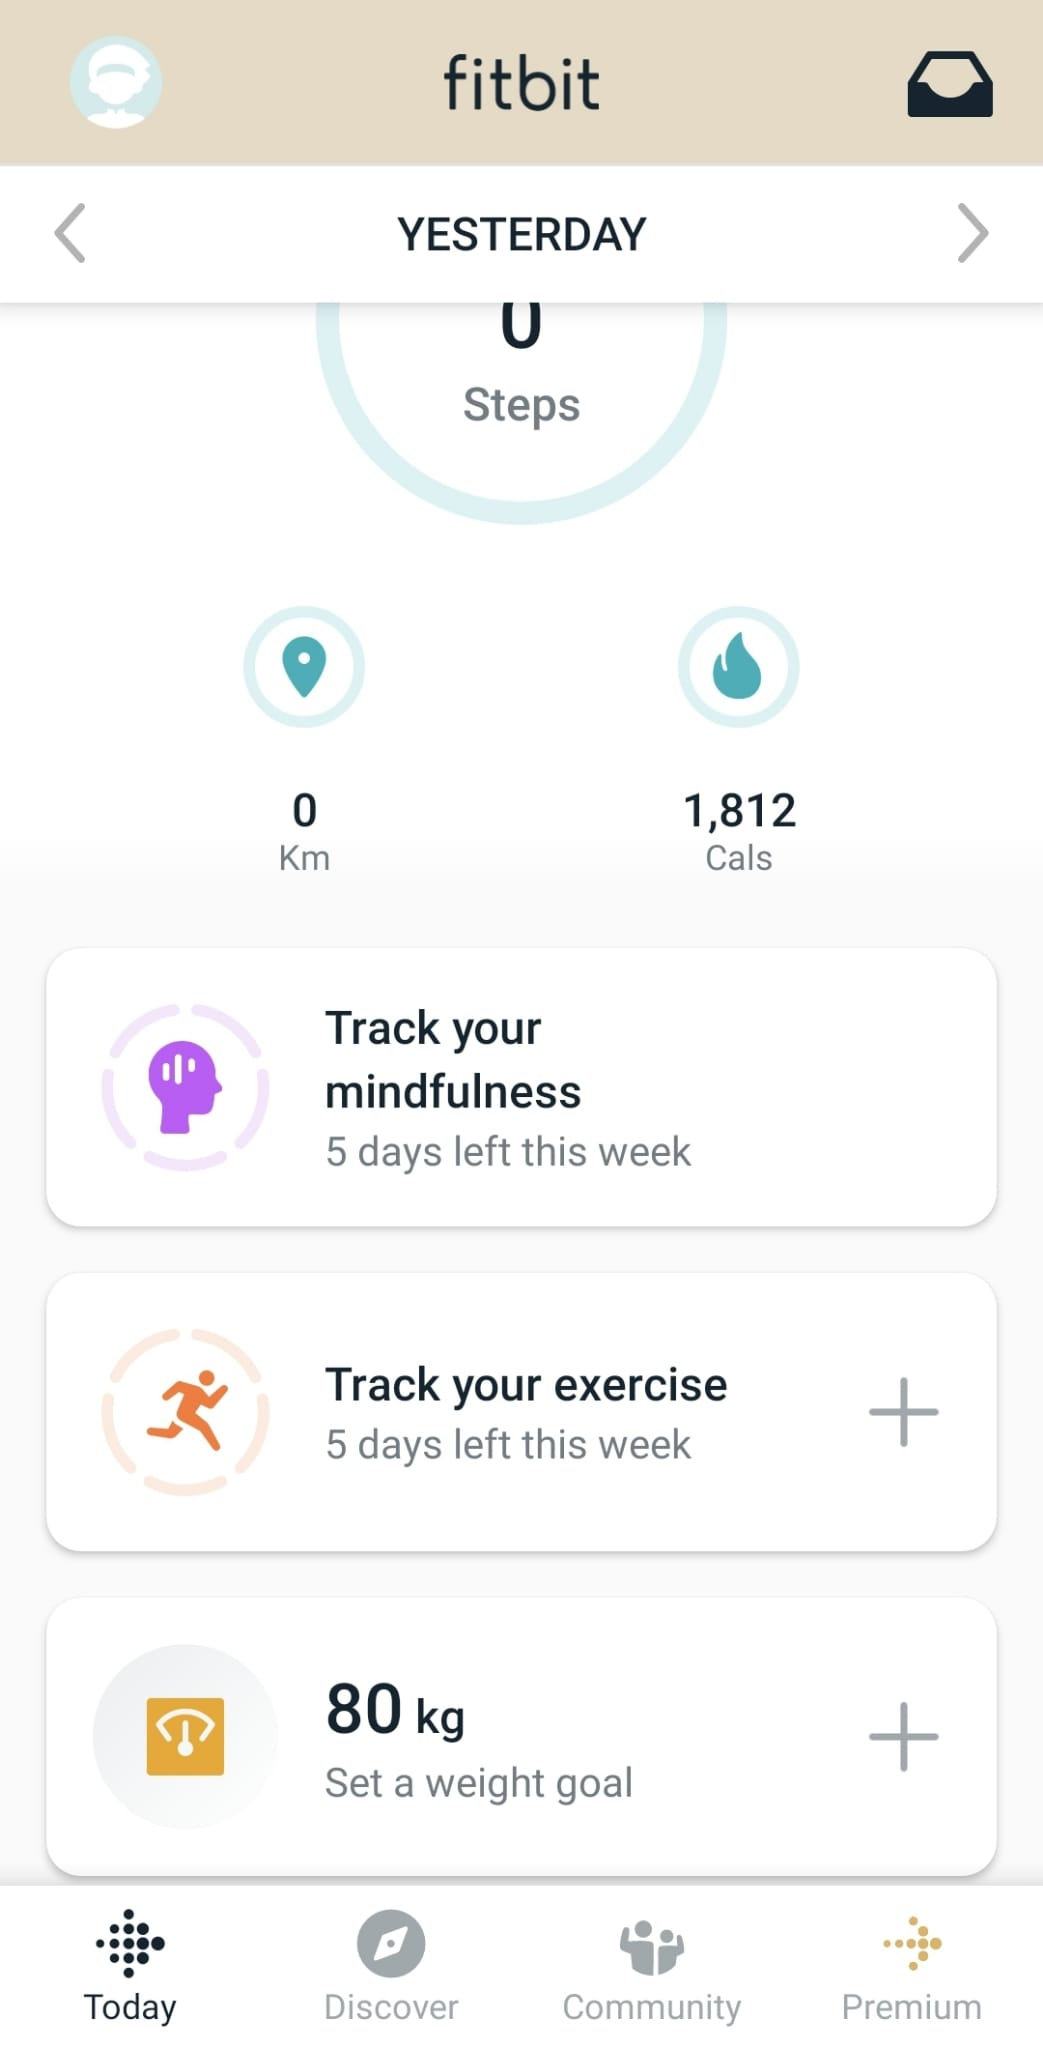
\includegraphics[width=0.5\textwidth]{fitbit/dashboard.jpeg}
        \caption{Dashboard}
        \label{fig:fitbit-home}
    \end{minipage}%
    \begin{minipage}{0.5\textwidth}
        \centering
        
\includegraphics[width=0.5\textwidth]{fitbit/food-tracker.jpeg}
        \caption{Food log screen \& features}
        \label{fig:fitbit-log}
    \end{minipage}
\end{figure}
\textbf{User Story}
\label{research-breakdown:fitbit-usr-story}
\par
``As a professional athlete I wake up, go through guided meditation on my Fitbit calendar before weighing myself (\cref{fig:fitbit-home}).
I then log my breakfast and eat (\cref{fig:fitbit-log}), followed by my commute to practice
and logging my sport and duration (\cref{fig:fitbit-exercise-log}).''

\begin{figure}[H]
	\centering
	\includegraphics[width=0.25\textwidth]{fitbit/exercise-choice.jpeg}
	\caption{Using exercise search \& log}
	\label{fig:fitbit-exercise-log}
\end{figure}
\pagebreak


\textbf{Features/Functionality}
\label{research-breakdown:fitbit-features}
\par
Fibit includes all of the following features:
\begin{multicols}{2}
	\setlist{nolistsep}
	\begin{itemize}[noitemsep]
		\item Guided meditation (w/ simple week-calendar scheduling).
		\item Guided video workout plans (w/ simple week-calendar scheduling).
		\item Guided programmes (for meeting targets in health, not just fitness).
		\item Challenges (1-10 people, gamifying targets).
		\item Water tracking.
		\item Food tracking.
		\item Track exercise (only by sport/activity, no custom option and no individual exercises/routines).
		\item Step counter.
		\item Community feed and groups.
		\item Add friends and send/receive messages.
	\end{itemize}
\end{multicols}
\textbf{Technology Stack}
\label{research-breakdown:fitbit-stack}
\par
Fitbit uses the following technologies according to Stackshare \cite{fitbit-stack}:
\begin{itemize}
	\item JavaScript(and Ember.js) for the front end.
	\item Fastly (for cloud content delivery)
	\item Redis (for middle layer and database caching)
	\item Node.js (for producing backend APIs)
	\item Java (and Spring) for the non-mobile applications
	\item MySQL (for the backend database(s))
\end{itemize}
Fitbit is cross-platform and multifunctional, thus there will be some technologies
not in use by the mobile app we are researching. It's unlikely Spring
is in use, but the use of JavaScript (w/ Node.js) for the front and backend is
common in current world of software. It's highly likely
the whole system is using a microservice architecture where components maybe used in several places.
\pagebreak

\subsection{Comparing MyFitnessPal and Fitbit}
Firstly, we'll note that both applications make use of JavaScript for their front-end technologies.
It's difficult to pinpoint what is being used without decompiling both applications (both of which have a huge codebase).
It is apparent that MFP is using React\footnote{an open-source UI software framework created by Meta, Inc (formerly Facebook)}.
Both apps are also using some form of CDN to speed up content delivery, which is needed given the abundance of data involved in
the tracking of food and exercise. MFP offers developers access to their data set via their own API \cite{mfp-api}.
\par
Whilst both apps calculate calories burned (an arguably useless metric for \textit{our project})
during exercise. The scope and functionality of exercise is vastly different.
Fitbit includes general sports and activities but no specific exercises (for example
- ``weights'' is considered 1 exercise type and the calories burned are dependent on duration)
and there is no ability
to produce your own routine.
On the other hand, MFP allows for the creation (and sharing) of your own routines using their
database of exercises. There are no videos to follow for this component of the app.
Both apps do however offer workout routines (and short-term programmes) via 
short videos published by the respective companies.
\par
Both apps allow for the tracking of food and water intake, as well as the ability
to scan product barcodes to log nutritional information. In regard to overall wellness,
Fitbit seems to be covering more ``bases'' by providing guided meditation videos and challenges
which can be taken alone or as a group. These challenges are a way to gamify the achievement of
personal goals (such as using your phone less).
\par
Finally, both apps include community features - very similar to traditional social media platforms.
These and other nutrition focused features are beyond the desired scope of \textit{our project} \todo[]{Internal link to requirements} thus we won't be
comparing and considering these.
\par
Overall, the fitness aspect of MFP seems more useful, but there are elements of the app which are not yet
on par with Fitbit - such as the goal setting and mindfulness measurements. 
That said, the UX/UI of MFP is more usable and the app has fewer features locked behind hardware devices
(yet you can still pair compatible devices to MFP). Neither app has any major feature involving the camera besides
the barcode scanning components. A combination of elements from both apps will be paramount to a successful project.
\par

\textit{The project} 
\todo[color=green]{reference prelim work}
is planned to have a side panel menu and similar minimal aesthetic to that of MFP.
It's not planned that it will include the calories burned estimates; however other metrics will be included in similar vain, such
as total time trained and cumulative weight lifted/cumulative distance travelled. Calorie estimates will be an enhancement (additional feature) where time permits.
The abilities to create custom routines and follow preset routines that are featured in MFP and Fitbit respectively,
are expected to be important features in \textit{the project}. Albeit, the long term plan for
things includes the ability for trainers to set these programmes as opposed to presets alone. 
\par
In summary, the design
and layout of these apps is what's useful for us - inspiration and additional features can also be drawn
from these existing systems. With that said, \textit{our product} is not a nutrition tracker and focusing
on elements in this space would shift the scope of the \textit{project} substantially. An extensive
breakdown of the feature set can be found in \cref{chap:project-specification}.\todo[color=yellow]{reference feature set}
\pagebreak
\subsection{TrueCoach}
TrueCoach provide a cross-platform system that includes a web application.
We'll be considering the mobile app provided for end users and making reference
to the functions available to administrators in the process. They provide a mobile app
for each of these use cases - ``\textbf{TrueCoach for Clients}'' and ``TrueCoach Connect'' for trainers.
\begin{figure}[H]
	\centering
	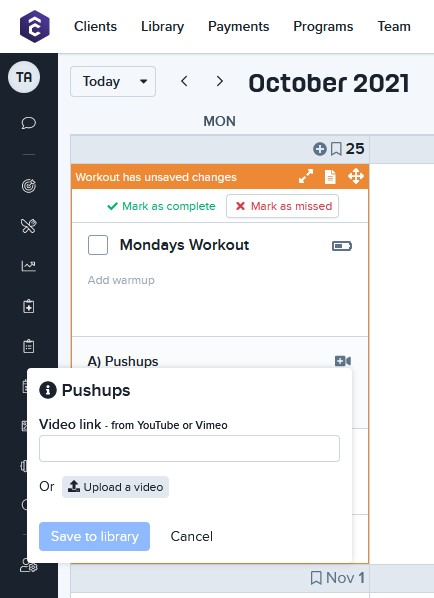
\includegraphics[width=0.3\linewidth]{truecoach/setting-client-workout.jpg}
	\caption{Trainer using web app to set clients workout(s).}
	\vspace*{-5mm}
	\label{fig:tc-trainer-set}
\end{figure}
\begin{figure}[H]
	\centering
	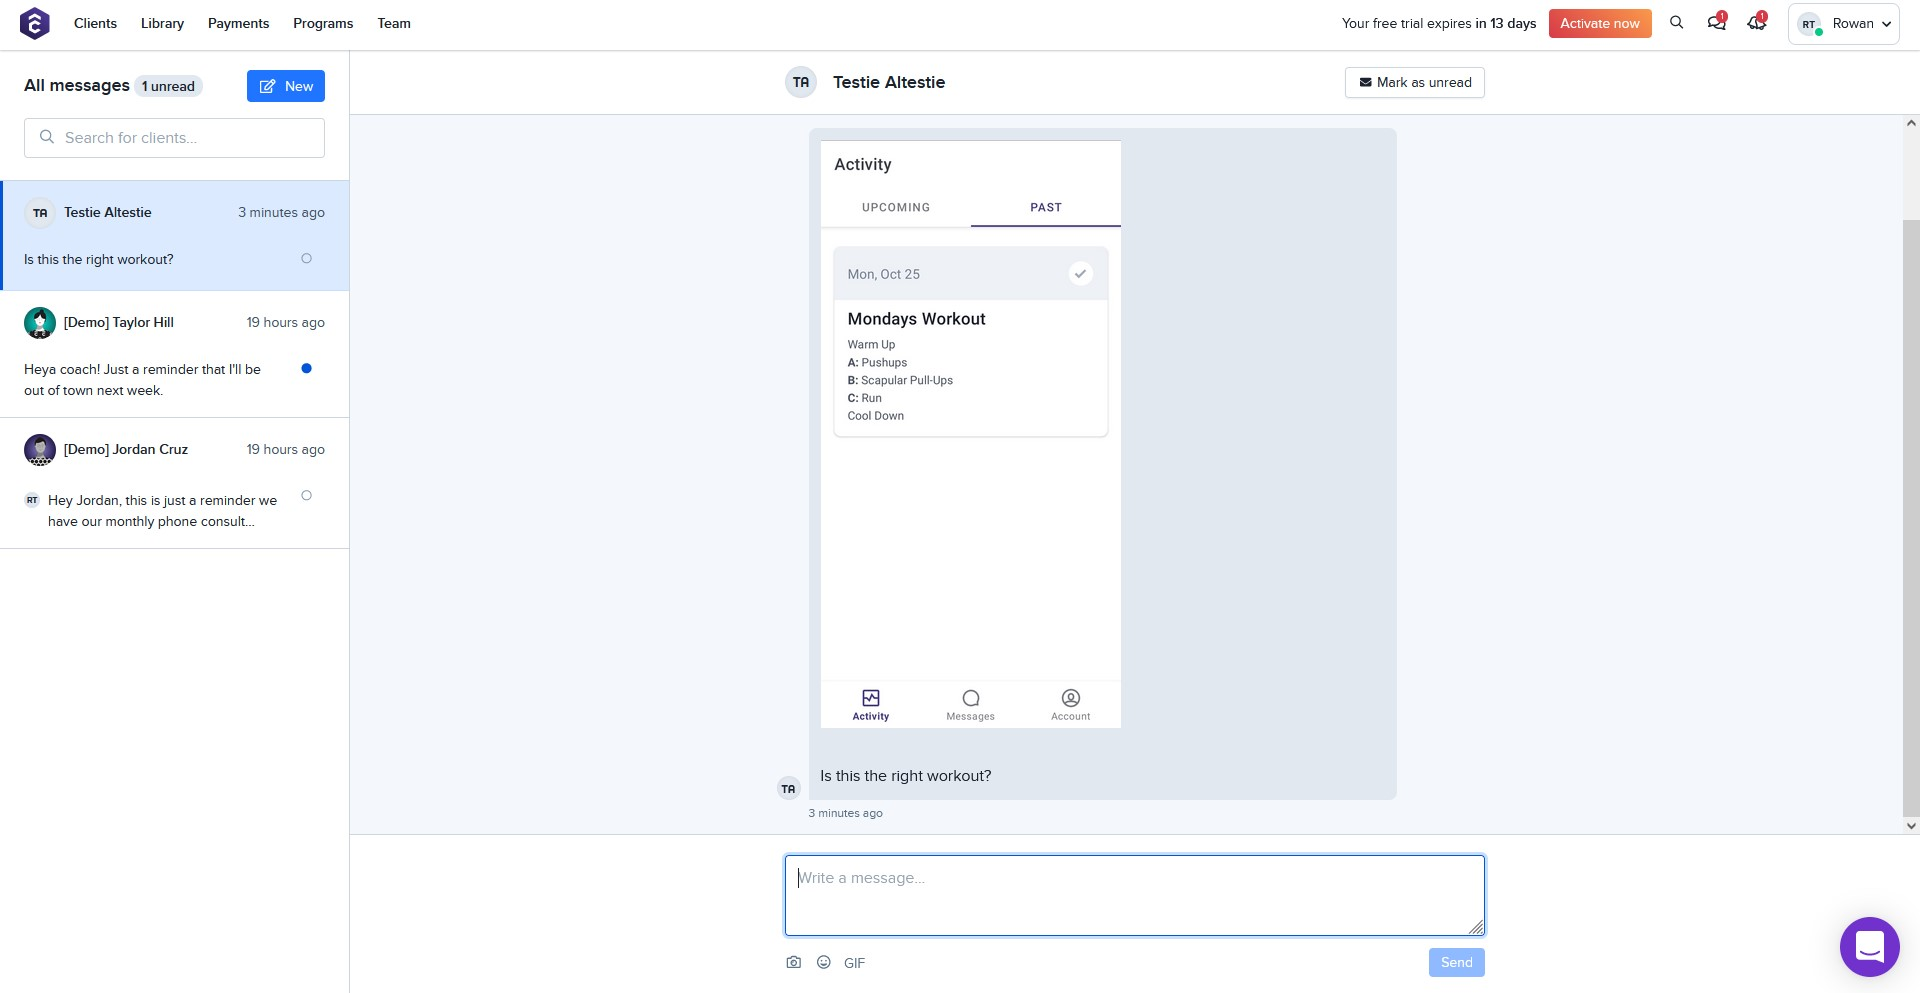
\includegraphics[width=1\linewidth]{truecoach/truecoach-web-chat.jpg}
	\caption{Trainer using web chat to manage clients.}
	\vspace*{-5mm}
	\label{fig:tc-trainer-chat}
\end{figure}
\textbf{User Story}
\label{research-breakdown:tc-usr-story}
\par
``As a new gym go-er, I work remotely with my trainer (\cref{fig:tc-trainer-chat,fig:tc-user-chat}) to refine my training technique(s).
I view my upcoming workouts (\cref{fig:tc-activity}) and follow instructional videos before marking my workouts as complete and monitoring 
my progress via goals \& challenges (\cref{fig:tc-workout}). For advice I can view
documents and progress photos in my settings page (\cref{fig:tc-settings}).''
\begin{figure}[H]
    \centering
    \begin{minipage}{0.4\textwidth}
        \centering
        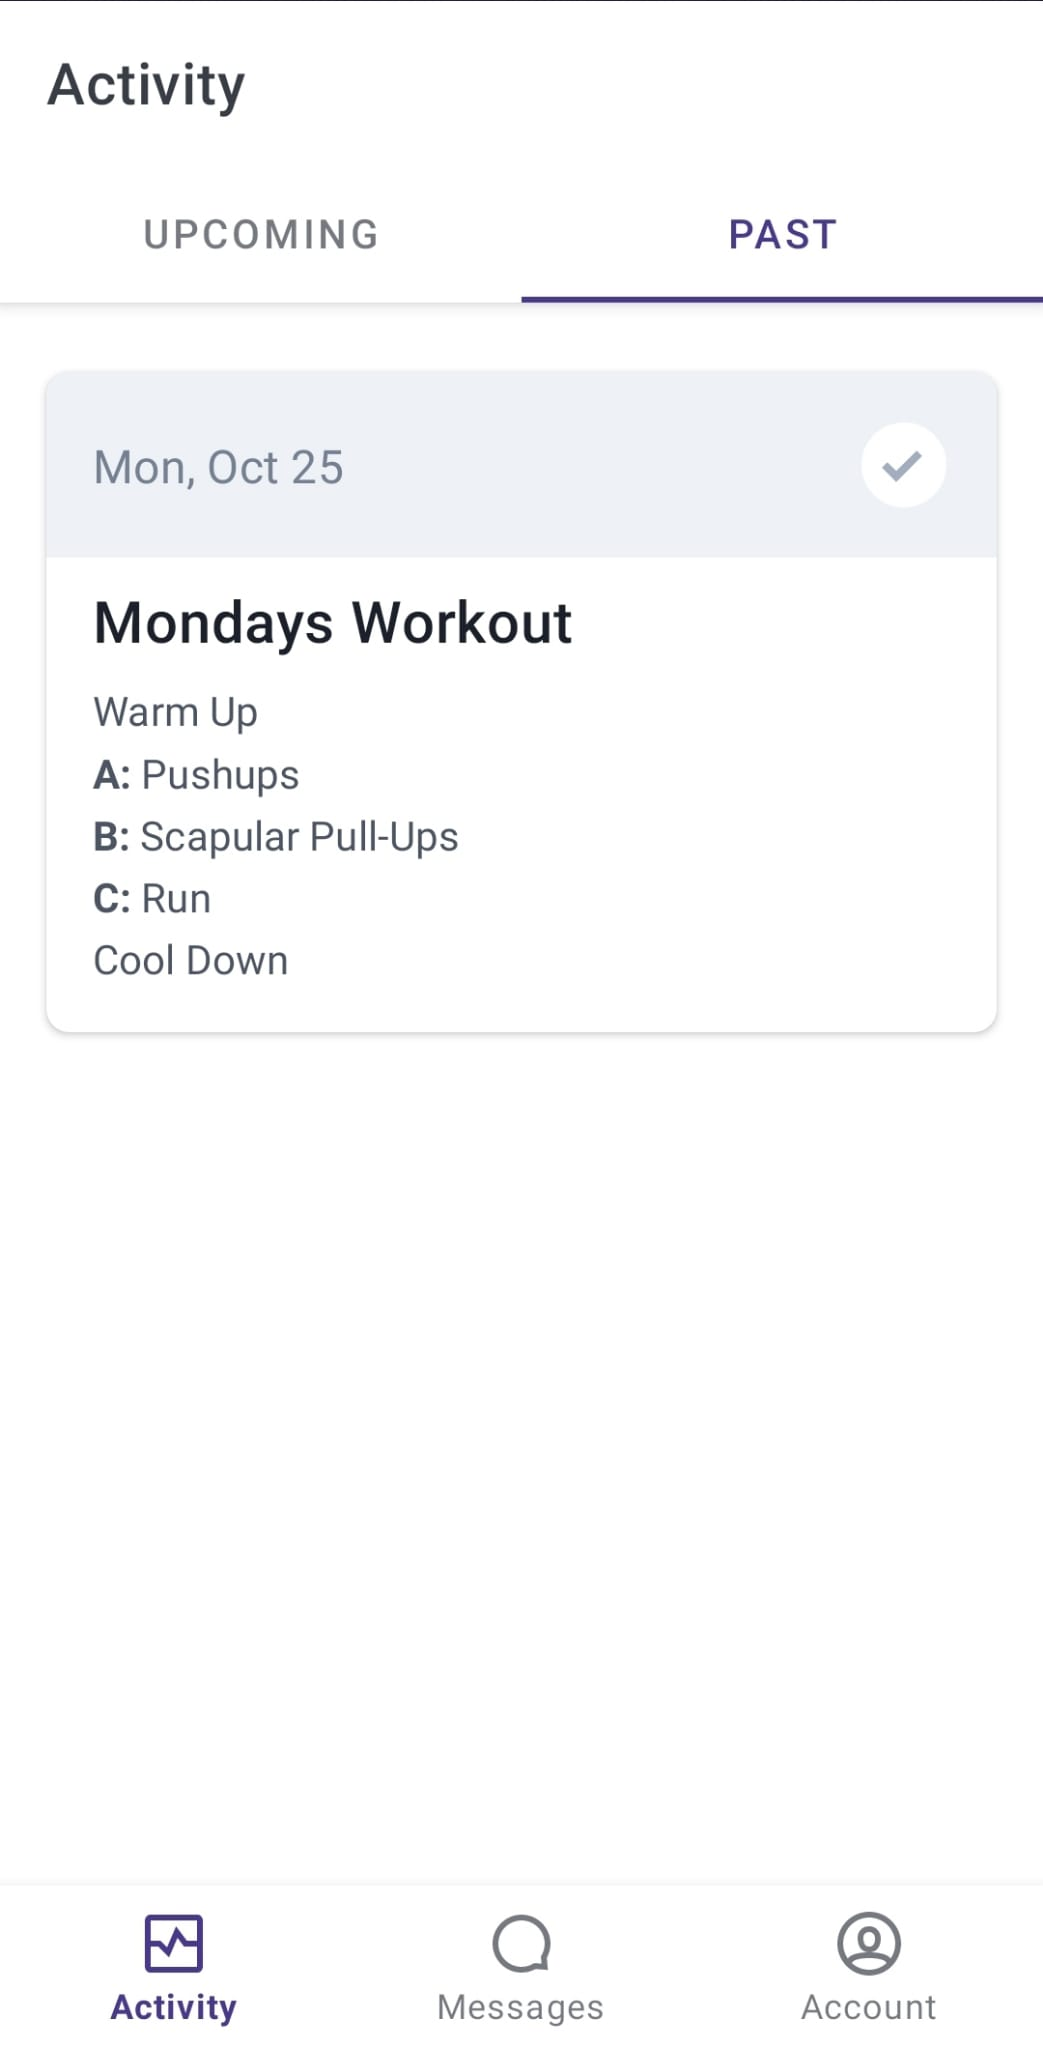
\includegraphics[width=0.5\linewidth]{truecoach/activity-page.jpeg}
        \caption{Viewing workouts (upcoming/past).}
        \label{fig:tc-activity}
    \end{minipage}\qquad
    \begin{minipage}{0.4\textwidth}
        \centering
        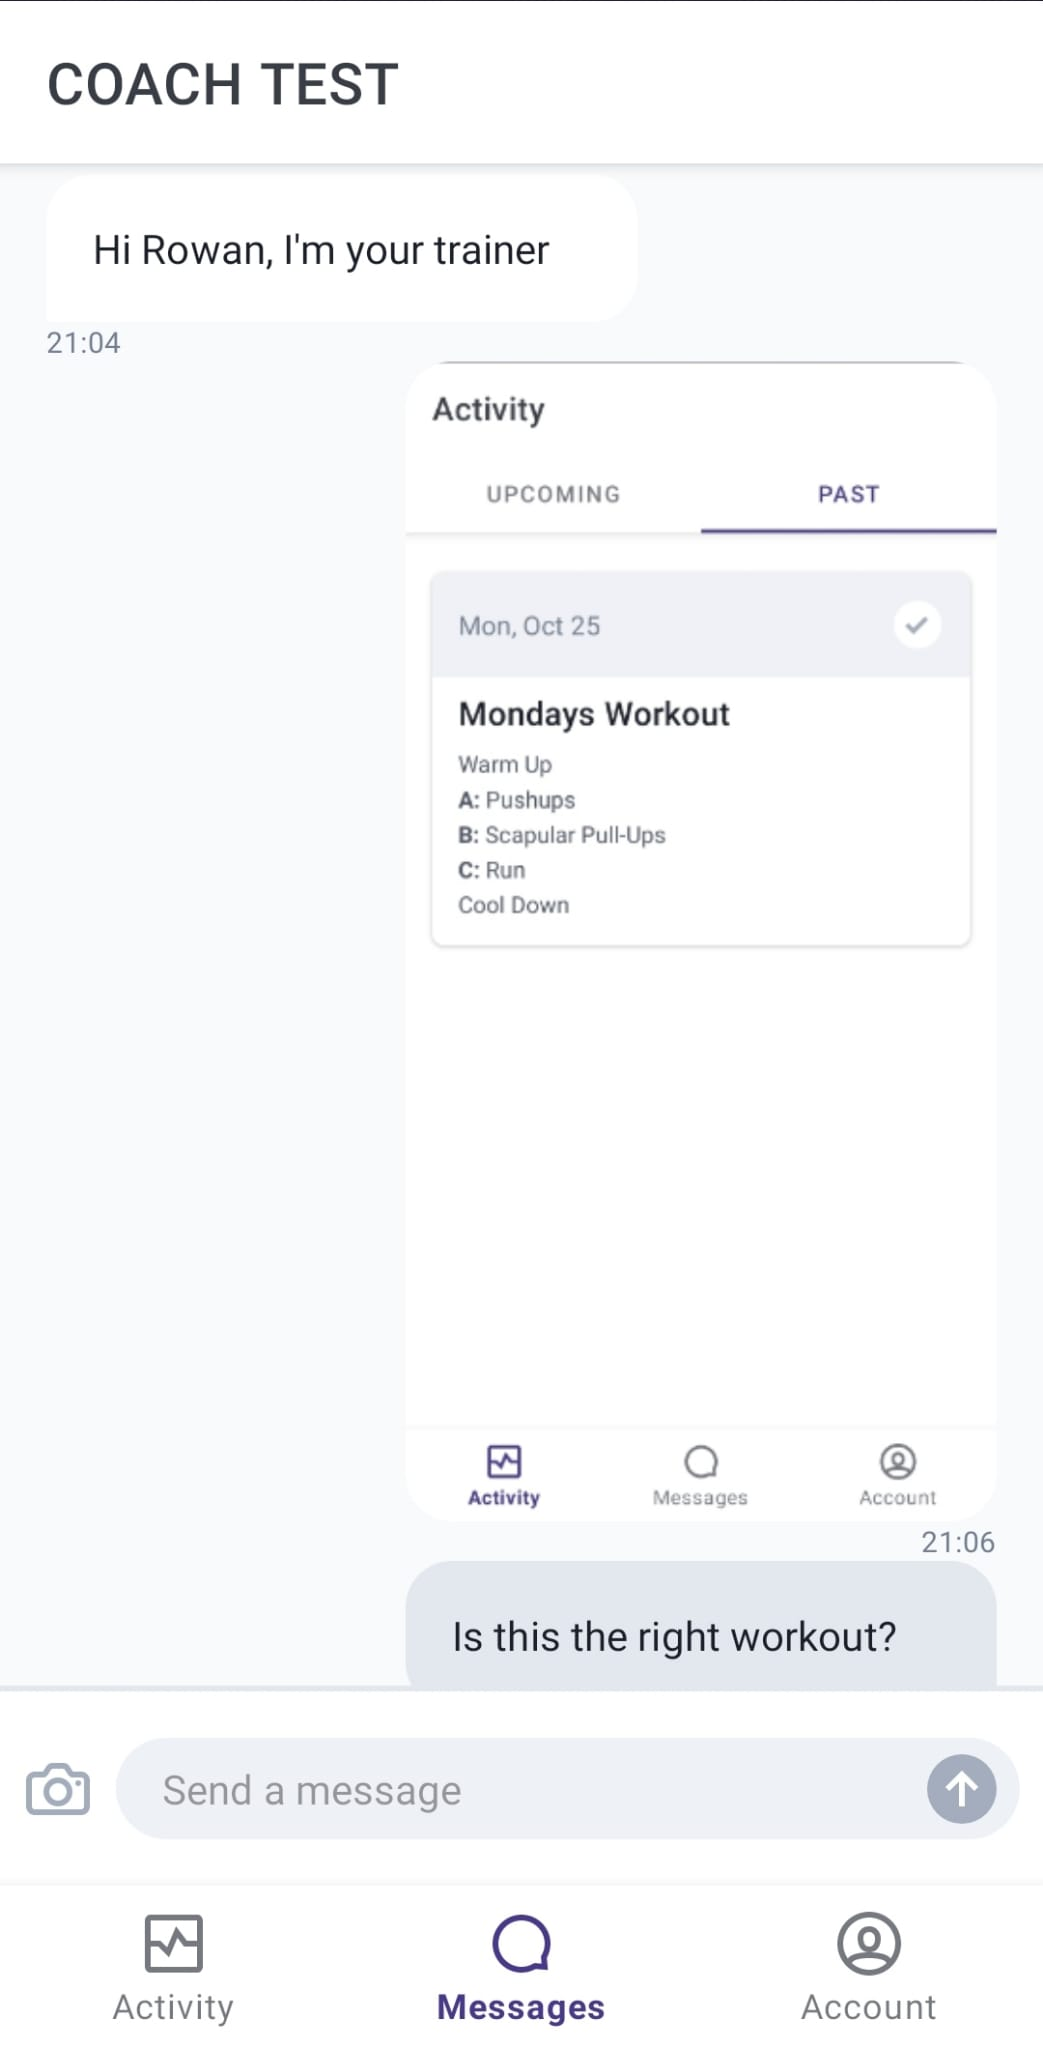
\includegraphics[width=0.5\linewidth]{truecoach/trainer-chat.jpeg}
        \caption{Instant messaging with a trainer.}
        \label{fig:tc-user-chat}
    \end{minipage}%
\end{figure}
\vspace*{-5mm}
\begin{figure}[H]
    \centering
    \begin{minipage}{0.4\textwidth}
        \centering
        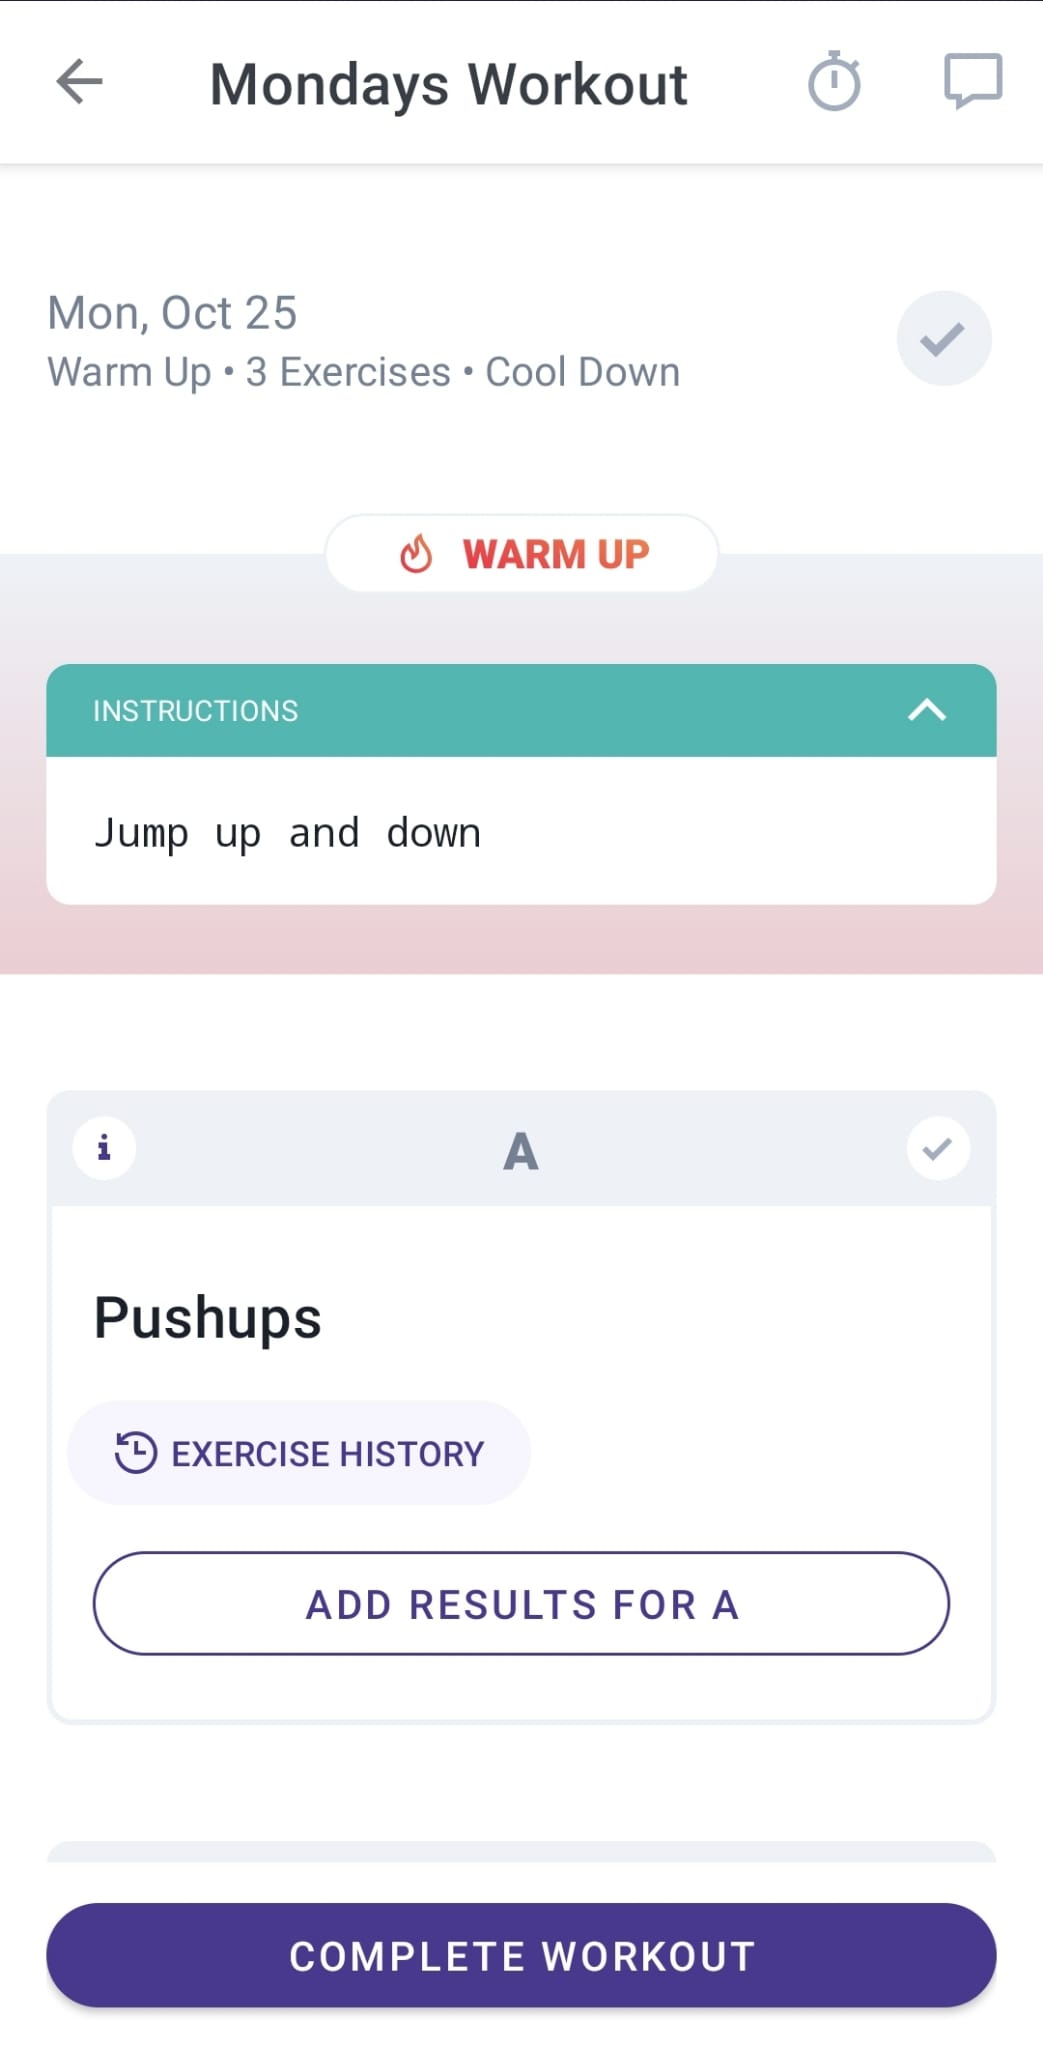
\includegraphics[width=0.5\linewidth]{truecoach/workout-logging.jpeg}
        \caption{Logging a workout.}
        \label{fig:tc-workout}
    \end{minipage}\qquad
    \begin{minipage}{0.4\textwidth}
        \centering
        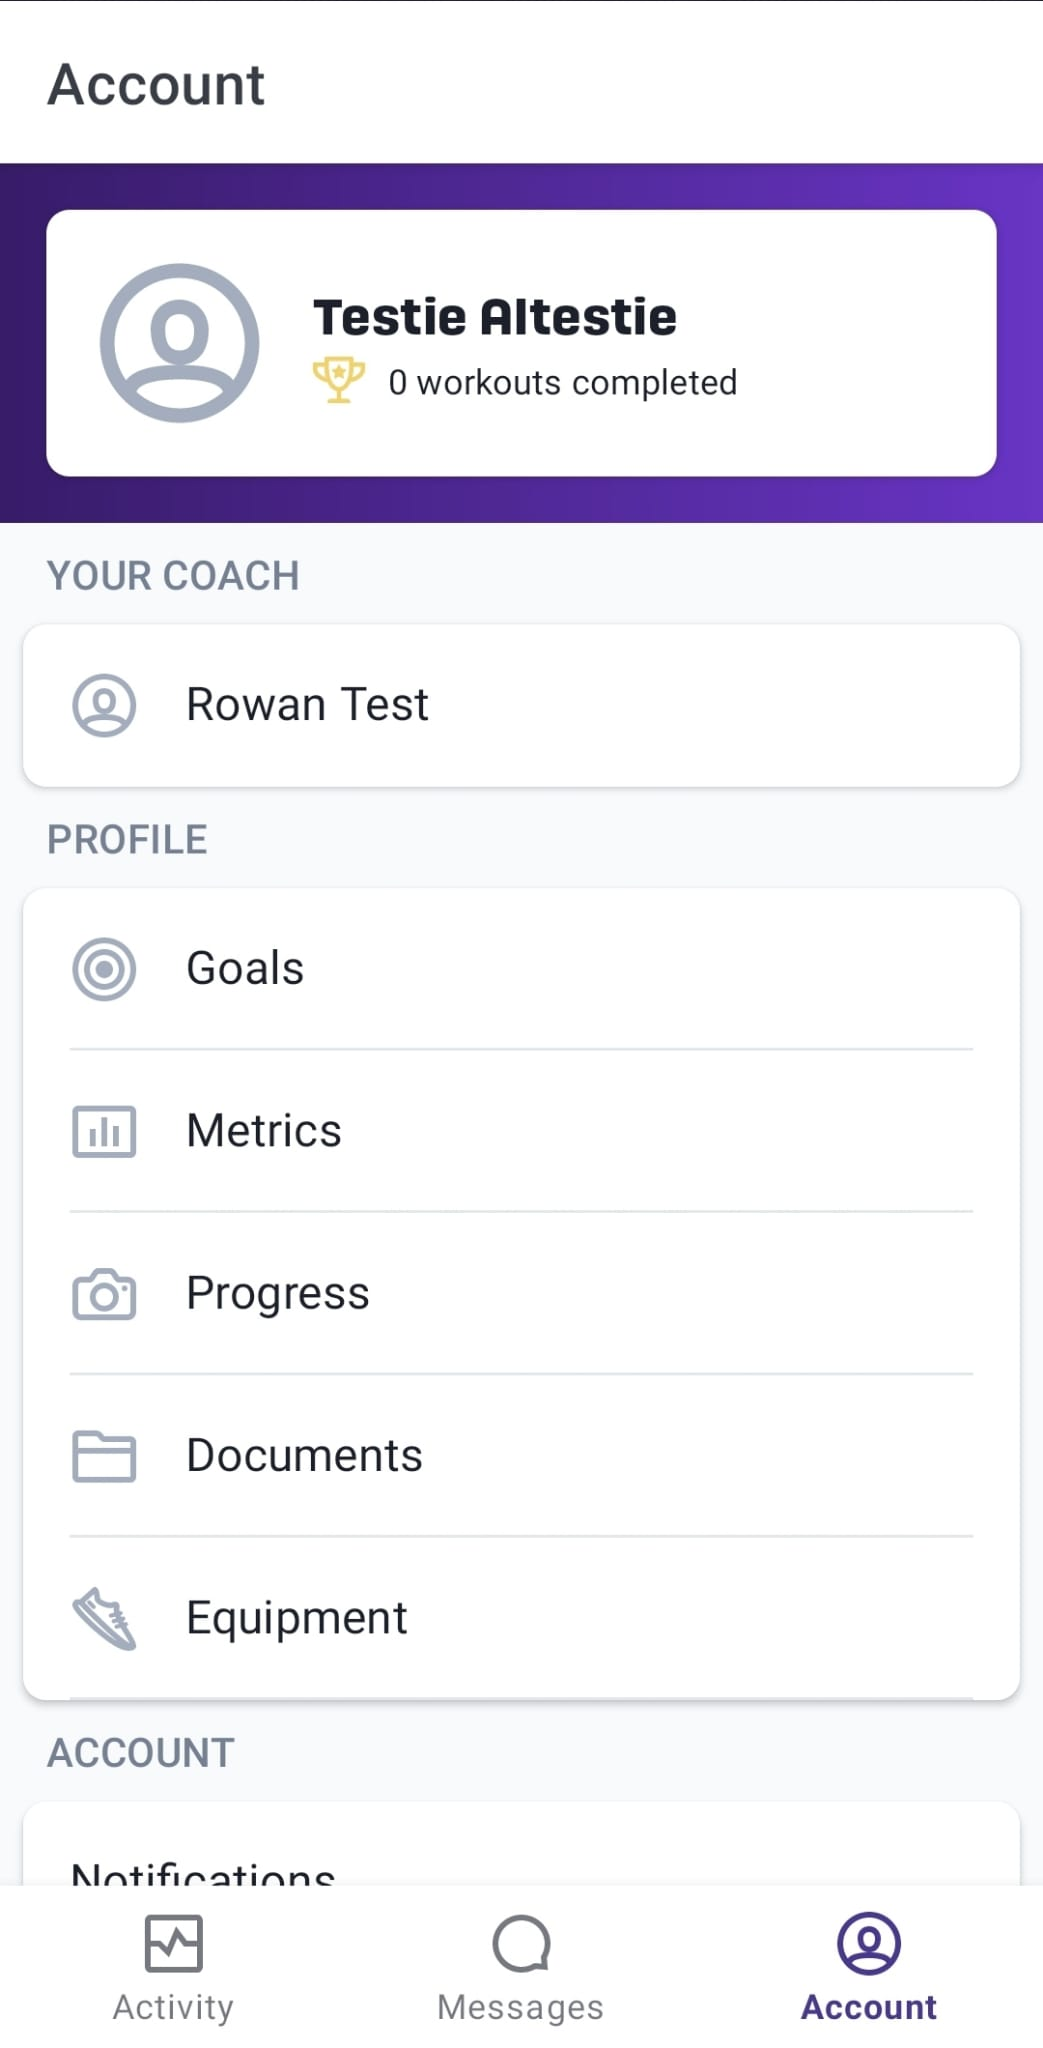
\includegraphics[width=0.5\linewidth]{truecoach/settings.jpeg}
        \caption{Viewing settings.}
        \label{fig:tc-settings}
    \end{minipage}%
\end{figure}
Above, ``Testie Altestie'' represents an end user and ``Rowan Test'' is the trainer. We can see
the functions available to the user are dependent on the workouts uploaded/scheduled
by the trainer using their interface (web application in this case).
\pagebreak

\textbf{Features/Functionality}
\label{research-breakdown:tc-features}
\par
\textbf{``TrueCoach for Clients''} includes all of the following features:
\begin{multicols}{2}
	\setlist{nolistsep}
	\begin{itemize}[noitemsep]
		\item Track coach's release of phased training (upcoming/past workouts).
		\item Log workouts (w/ notes).
		\item Timer \& stopwatch function for tracking timed exercises.
		\item Video breakdowns of exercises (w/ rich text instructions).
		\item Instant messaging w/ trainer (including multimedia uploads).
		\item Tracking of progress via trainer-set goals \& metrics.
		\item Progress and additional documents (outbound link to web app).
		\item Create account via invite link from trainer.
		\item View notifications.
		\item Edit settings (outbound link to web app).
	\end{itemize}
\end{multicols}
\vspace*{-5mm}
TrueCoach covers a lot of needs for a user, and we can see in \cref{fig:tc-trainer-chat} 
the relevant tools for the trainer to facilitate these workouts. They are administrators of their
clients and they're the means by which a user gets login credentials. 
Trainers can upload relevant videos (\cref{fig:tc-trainer-set}) and documents, as well as provide metrics
to measure users progress.
\par
\textbf{Technology Stack}
\label{research-breakdown:tc-stack}
\par
Stackshare (as used for the previous apps) is not useful in this case, so the following conclusions have
been drawn following the decompilation of the TrueCoach APK \cite{apk-decompiler}:
\setlist{nolistsep}
\begin{itemize}
	\item Kotlin \& Java (for Android development)
	\item Firebase (for push notifications and messaging)
	\item AWS Amplify (for backend deployment)
	\item Numerous open-source development packages such as \href{https://github.com/bumptech/glide}{glide}. 
\end{itemize}
After decompiling and opening the class files using \href{https://github.com/pxb1988/dex2jar}{dex2jar} and
\href{https://java-decompiler.github.io/}{JD-GUI}, I found that the application is not using a cross-platform
JavaScript framework as is standard in modern times. The app is using the recommended native language
of Kotlin\footnote{Learn more: \href{https://developer.android.com/kotlin}{android development documentation}} and Java for all data objects and frontend display. 
\pagebreak

\subsection{Exercise.com}
Exercise.com are the company providing the white-labelled solution behind \href{https://online.pjfperformance.net/users/sign_in/}{PJFPerformance}.
We'll be using the \textbf{PJFPerformance} app to analyse their application.
\begin{figure}[H]
    \centering
    \begin{minipage}{0.5\textwidth}
        \centering
        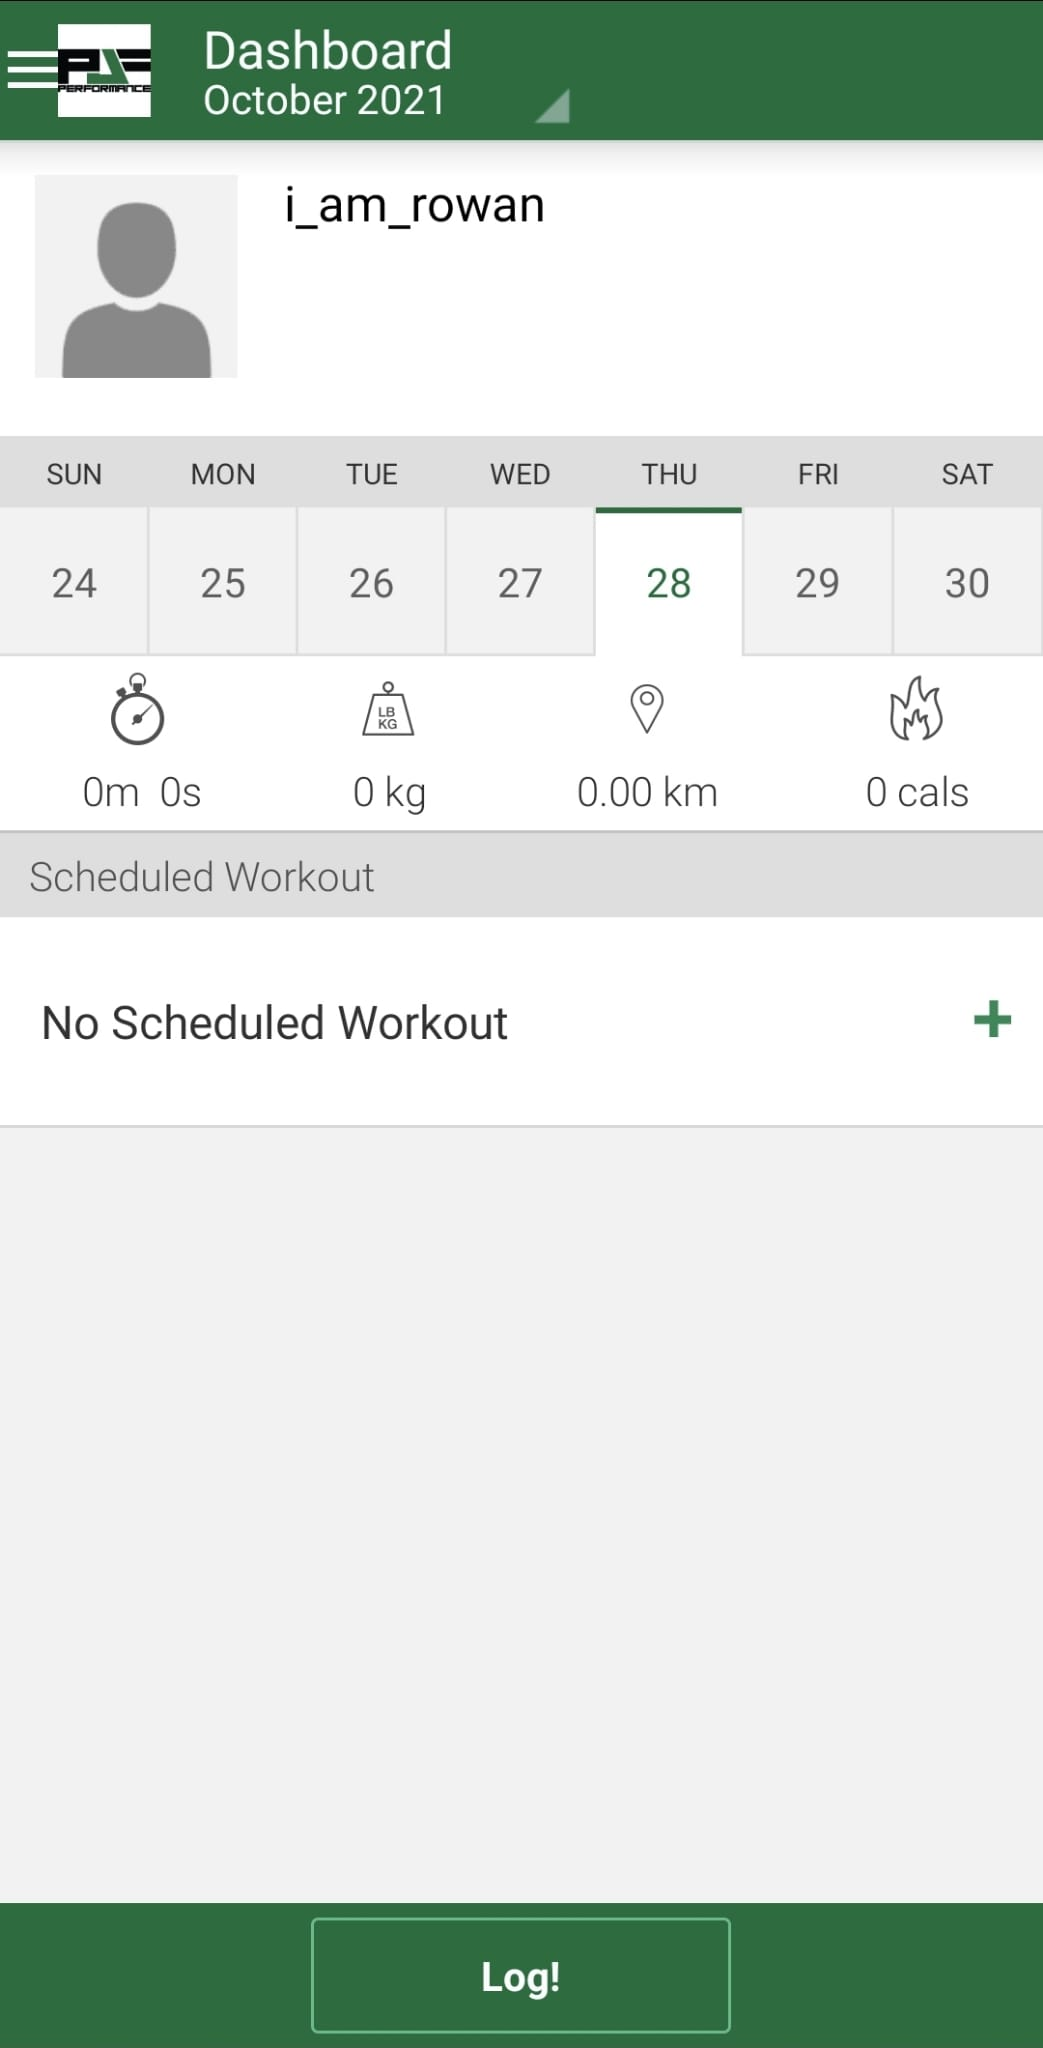
\includegraphics[width=0.5\textwidth]{pjf/pjf-dashboard.jpeg}
        \caption{Home dashboard}
        \label{fig:pjf-home}
    \end{minipage}%
    \begin{minipage}{0.5\textwidth}
        \centering
        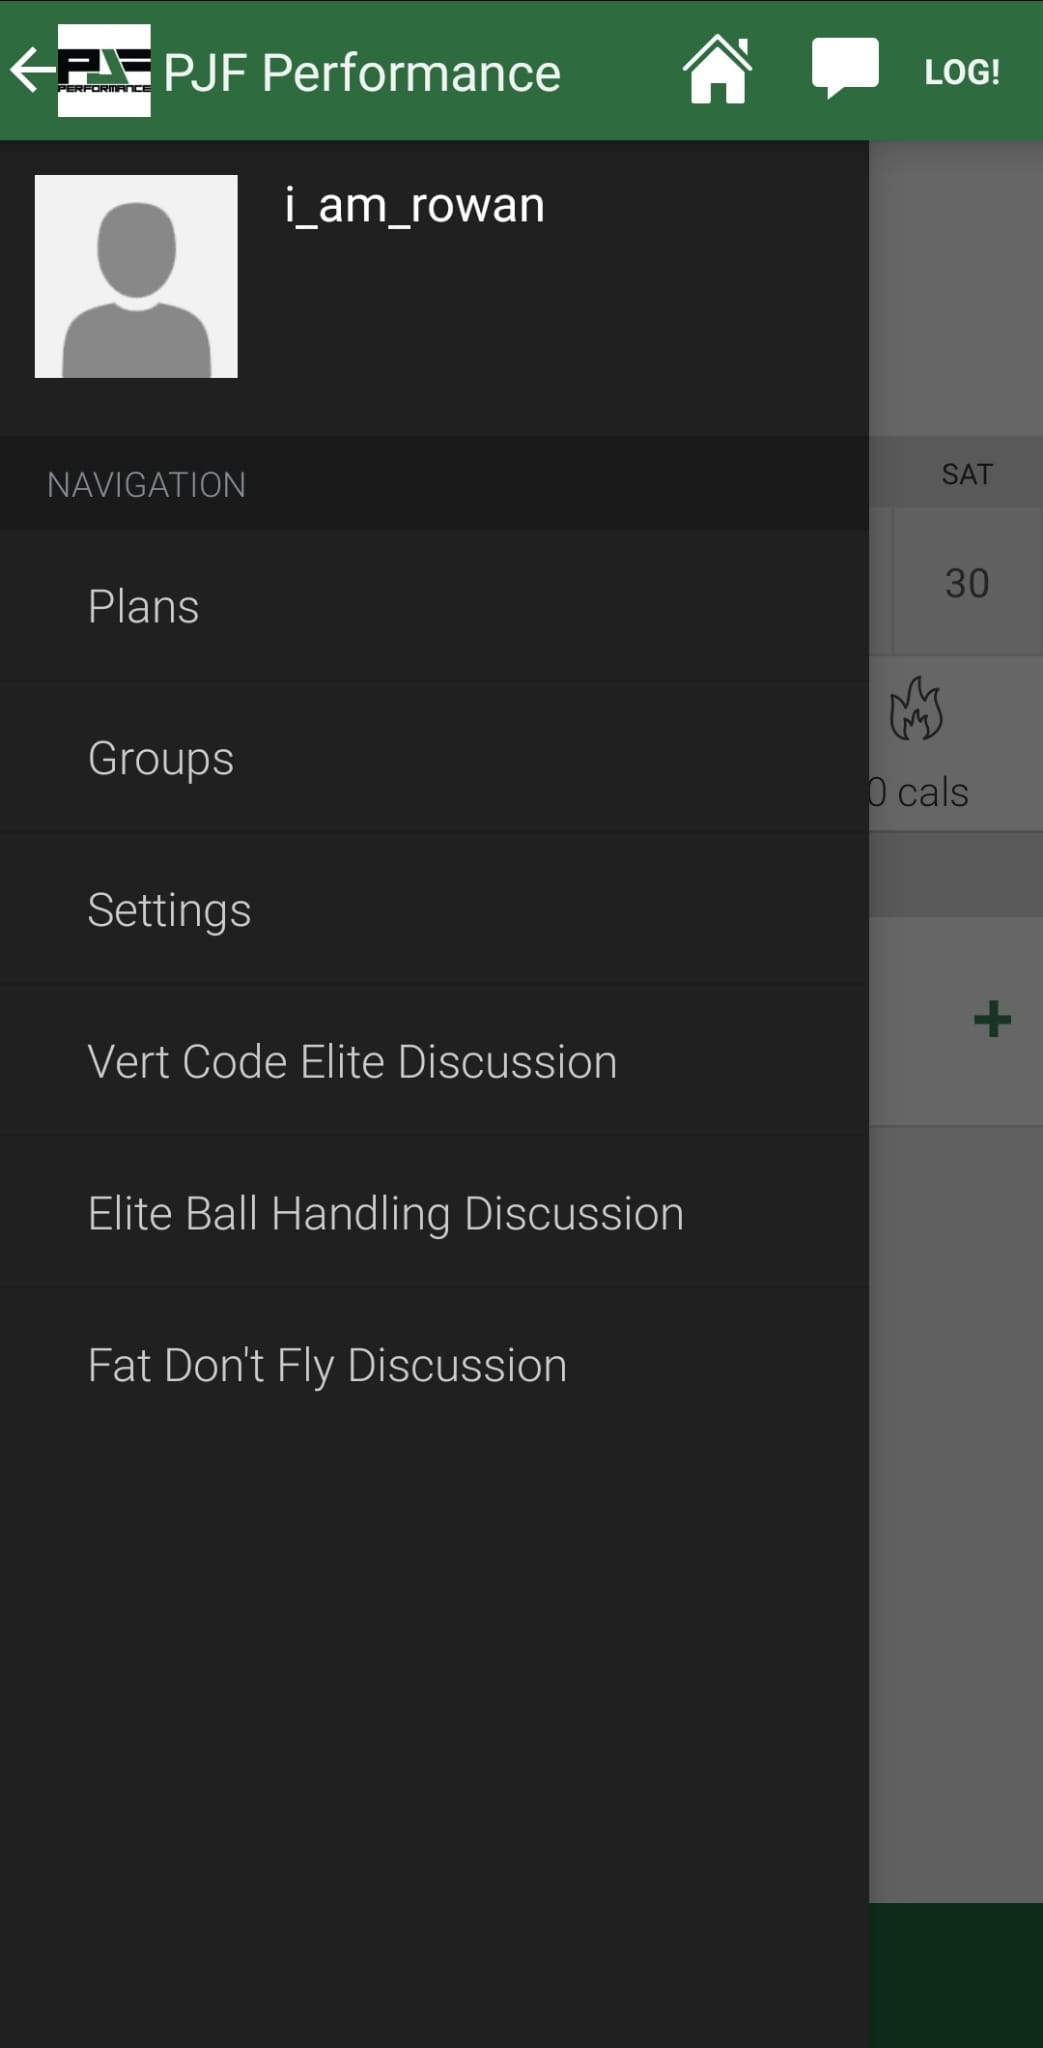
\includegraphics[width=0.5\textwidth]{pjf/pjf-menu.jpeg}
        \caption{Sidebar menu options}
        \label{fig:pjf-menu}
    \end{minipage}%
\end{figure}
\begin{figure}[H]
    \centering
    \begin{minipage}{0.5\textwidth}
        \centering
        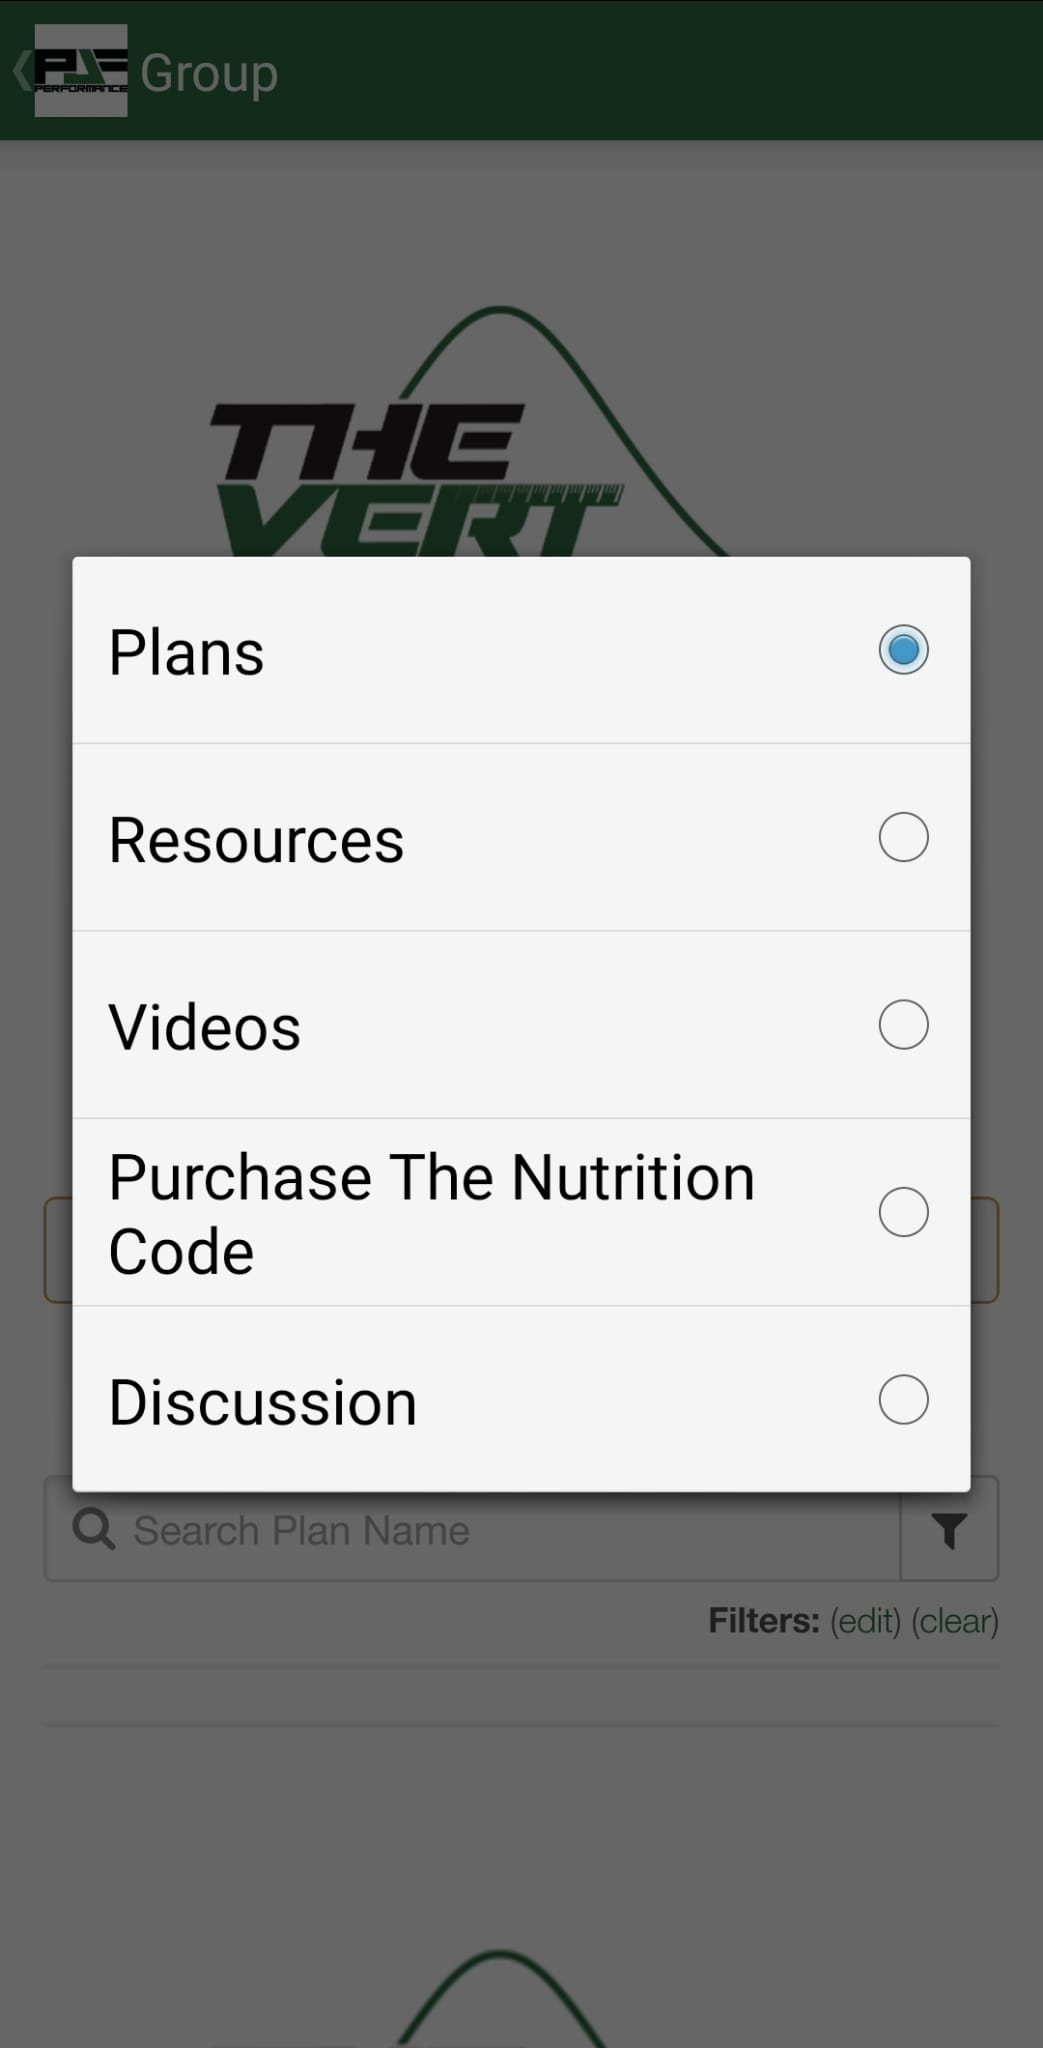
\includegraphics[width=0.5\textwidth]{pjf/pjf-group-resources.jpeg}
        \caption{Viewing additional resources.}
        \label{fig:pjf-resources}
    \end{minipage}%
    \begin{minipage}{0.5\textwidth}
        \centering
        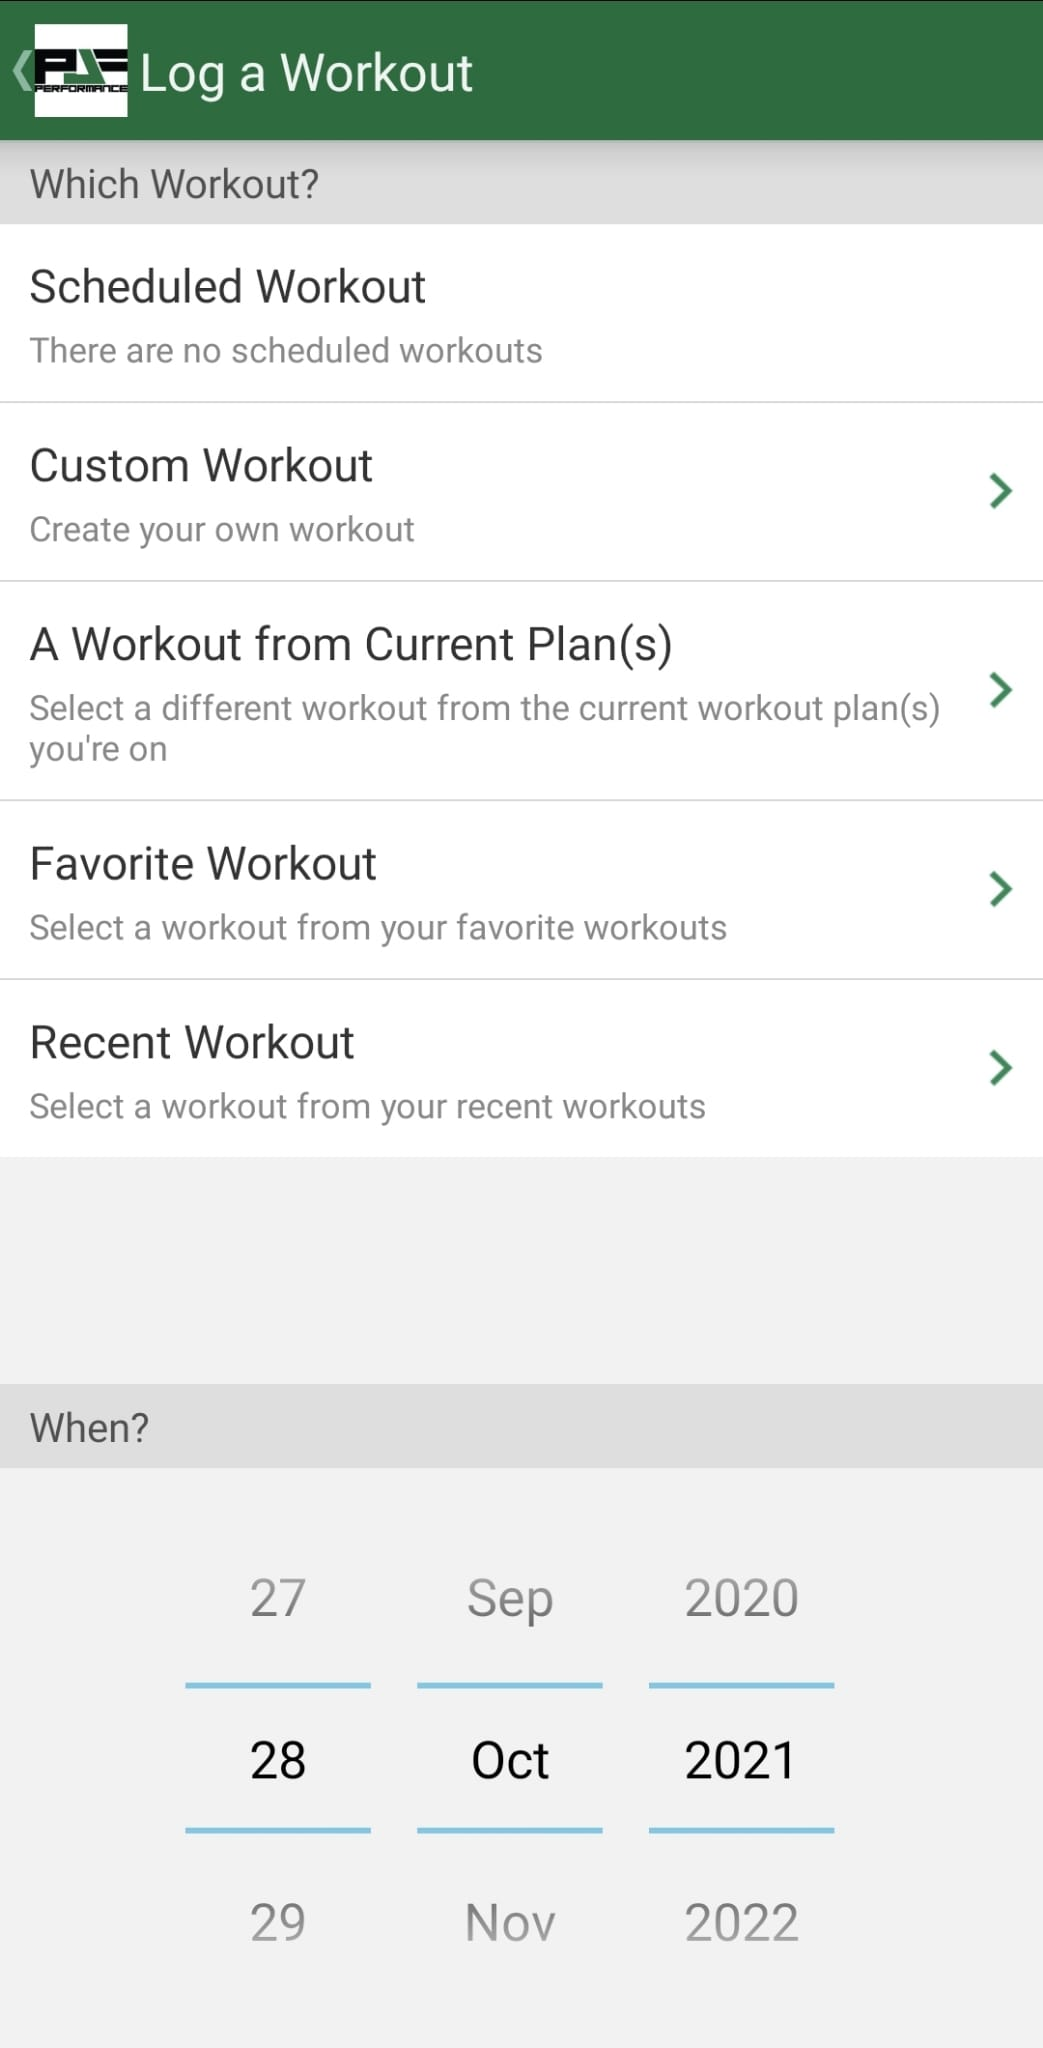
\includegraphics[width=0.5\textwidth]{pjf/pjf-logging-workout.jpeg}
        \caption{Scheduling/logging a workout.}
        \label{fig:pjf-workout}
    \end{minipage}%
\end{figure}
\pagebreak
\textbf{User Story}
\label{research-breakdown:pjf-usr-story}
\par
``As a basketball player, I enroll to Paul Fabritz' workout plan using the web application before
receiving credentials for the mobile app. Here I schedule the programme to begin
at the start of the month and I allocate days of the week for my workouts (\cref{fig:pjf-home}).
I create my profile containing my weight and other metrics, so I can ask relevant questions
to Paul and others on the same programme as me via a discussion room (\cref{fig:pjf-menu}). For guidance on training
during the season and managing load, there is a resources section (\cref{fig:pjf-resources}) (outbound links). I log all my workouts and make notes
for my own use. I sometimes create workouts for myself (\cref{fig:pjf-workout}) using some exercises available through the app.
Whenever I train, I can see exercises explained via videos embedded from YouTube.''

\textbf{Features/Functionality}
\label{research-breakdown:pjf-features}
\par
The PJFPerformance app includes all of the following features:
\begin{multicols}{2}
	\setlist{nolistsep}
	\begin{itemize}[noitemsep]
		\item Schedule workouts.
		\item Create custom workouts (using existing exercises).
		\item Log workouts (w/ notes).
		\item Enroll on phased programmes (made up of multiple workouts split over
		a given number of weeks \& days).
		\item Edit profile.
		\item View settings.
		\item View notifications.
		\item Rest timer for timed sets in workouts.
		\item Videos (YouTube hosted) for exercises.
		\item Group discussions for programmes.
		\item View additional resources (hosted externally).
	\end{itemize}
\end{multicols}
\vspace*{-5mm}
Exercise.com work on a 1-to-1 basis with trainers and white-label their solutions, this means
any administrator view can only be presumed via the decompilation of the APK app file.

\textbf{Technology Stack}
\label{research-breakdown:pjf-stack}
\par
Similarly to \hyperref[research-breakdown:tc-stack]{TrueCoach}, finding the technology used by Exercise.com for the mobile application is only possible
via decompilation using existing tools \cite{apk-decompiler}.
Based on my look into the source code, we can safely conclude that the app uses:
\setlist{nolistsep}
\begin{itemize}
	\item Kotlin \& Java (for Android development)
	\item Firebase (for push notifications and messaging)
	\pagebreak
	\item Amazon S3 (for data storage)
	\begin{itemize}
		\item They expose data from the S3 instance via their web application API.
		This is where the mobile application is pulling data from.
		\item The S3 instance  is using some form of SQL database (we know this based on SQL migration scripts in the source code).
	\end{itemize}
	\item Numerous open-source development packages such as \href{https://github.com/alibaba/fastjson}{FastJson}. 
\end{itemize}
Similarly to \hyperref[research-breakdown:tc-stack]{TrueCoach}
this app is written using Kotlin and not a cross-platform JavaScript framework.
The MaterialDesign\footnote{a design language invented by Google (Android parent company) in 2014.}
influence is noticeable in this app and so it is less surprising. Performance to the User
feels somewhere between average and slow for this type of app.

\subsection{Comparing TrueCoach and PJFPerformance (Exercise.com)}
TrueCoach has a larger focus on the client-trainer relationship and is more suited to
the public (anybody can become an administrator and begin using their platform for their business).
On the other hand, PJF provides a greater reliance on the community of people following the same 
programme as the User. Our project aims to blend both of these concepts; the core functionality will be developed first (focusing on the end user)
before producing administrator views and allowing a many-to-many relationship between clients and trainers.
\par
From a technical standpoint the implementation of the applications are similar (both using Kotlin and Java, with
some use of open-source packages for specific needs - such as confetti in TrueCoach when completing a challenge).
Both apps also make use of Firebase messaging for push notifications. This is easily implemented
and simplifies the implementation of push notifications across platforms (Android/iOS). This is noteworthy for
the development of our project and will prove useful if Firebase is used instead of or alongside the technologies outlined
in \cref{chap:project-specification}\todo[color=purple]{tech stack reference here}. Our application frontend will be built
using Flutter. The reasoning for this will be outlined further in the document, but performance is not expected to be adversely affected.
Whilst the technology will be different the functionality and user experience aims to be similar to that of both apps.
\par
TrueCoach has a simple 3 screens - logging and monitoring workouts (\cref{fig:tc-workout}) has a much better UX/UI.
The ability for a trainer to add new exercises and accompanying video
 (both via embeds or uploading raw video) is unique (\cref{fig:tc-trainer-set}). These are features that are
greatly beneficial to our project and reducing the number of app screens and keeping the interface minimal will
both provide a much better final product and ease the time stress of development and testing.
Only in the PJF app can a user create their own workout and log this (\cref{fig:pjf-workout}). This ability is
core to our app. On the other hand, the TrueCoach app is entirely dependent
on a trainer/administrator supporting you throughout your programme. Furthermore,
TrueCoach allows for the measurement of set metrics (by the trainer) and goals to surpass.
The PJF app lacks these features but does allow for further planning in the form of a calendar view and 
a ``traffic-light system'' for workouts on a daily basis. A red circle appears under missed workouts
on the calendar, amber for pending workouts for the day and green workouts for completed workouts. TrueCoach
has personal goals but no extensive calendar view and there is a simple ``mark as completed'' feature
for scheduled workouts. Both of these elements are planned to be included on our project; looking at the preliminary
prototype \todo[]{reference prototype} and feature set \todo[]{reference feature set} should provide more clarity on how this will be achieved.
\par
The final difference I consider notable between the apps is the use of timers. TrueCoach makes use of both
a stopwatch and a timer for users to utilise during exercises. Alternatively, PJF includes a rest timer
which Paul suggests to use for other functions but no stopwatch if needed (for example, when training for speed).
We plan on following TrueCoach's example here and allowing users the option of both. Implementation is relatively easy
 and should enhance user experience.
\par 
Many of the differences outlined above come down to the business objectives of the relative applications. TrueCoach is building a
SaaS company whereas Exercise.com is building a fitness application product that they can
white-label to notable trainers in the fitness industry. This core difference means there are certain
design decisions that differ between the apps. A common and core feature with both is the 
ability for users to view videos of exercises during workouts and to log there progress as they exercise.
This is important to the success of \textit{the product} and the approach we are looking at following involves
a dashboard upon registration where a trainer can include their branding and thereby personalise the end user
experience - similar to Stripe (\cref{fig:stripe-customization}).
\pagebreak

This functionality falls beyond the scope
of the outlined \textit{project} but will help you form a long-term understanding of the proposed system.
\par
There are many small differences both in the technologies used (such as AWS Amplify vs S3 storage and a self-hosted API)
and in the feature sets. Ultimately, elements of both applications should be used in 
\textit{the project} in order to produce a market-suitable \textit{product}.
\begin{figure}[H]
	\centering
	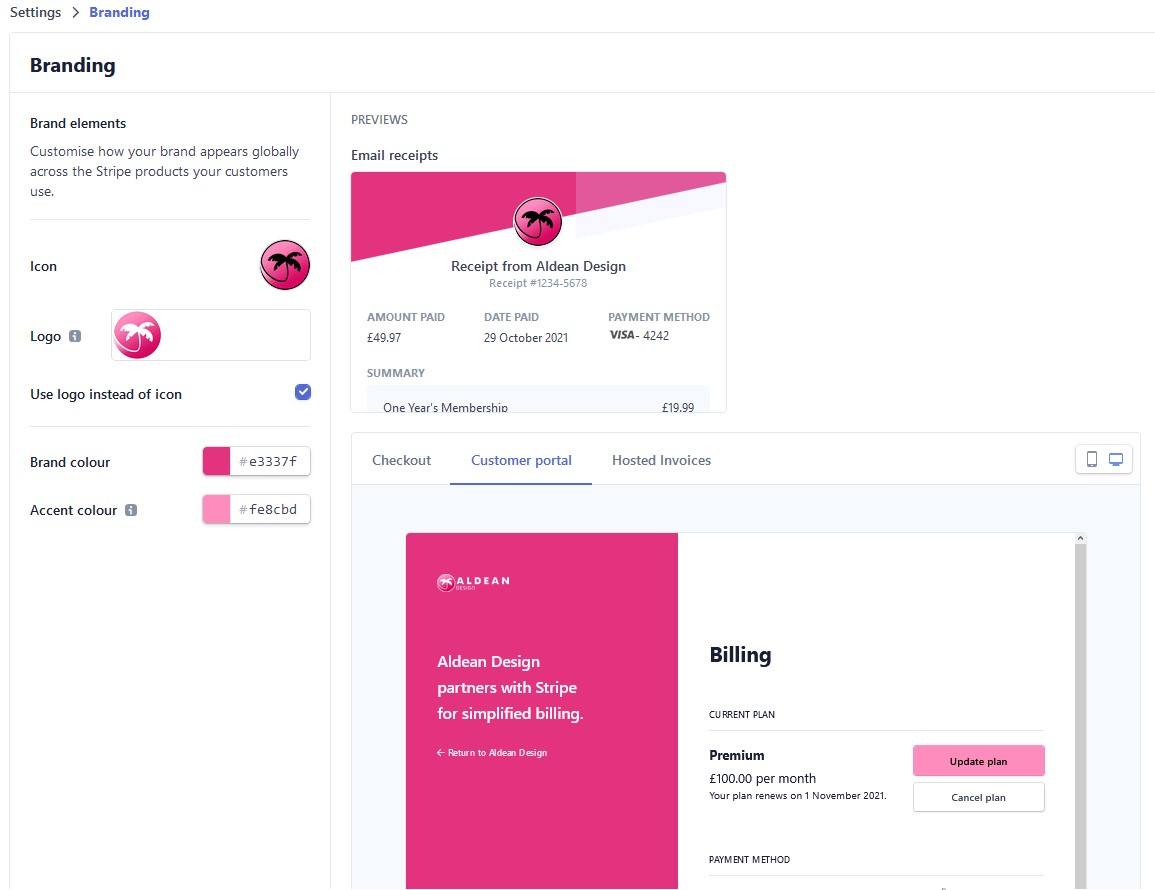
\includegraphics[width=1\linewidth]{graphics/stripe-customization.jpg}
	\caption{Customizing Stripe products using personal branding.}
	\vspace*{-5mm}
	\label{fig:stripe-customization}
\end{figure}
\pagebreak